\documentclass[10pt]{article}
\usepackage[margin=1in]{geometry}
\usepackage[utf8]{inputenc}
\usepackage{amsmath,amssymb,amsfonts}
\usepackage{algorithmic}
\usepackage{algorithm}
\usepackage{graphicx}
\usepackage{textcomp}
\usepackage{xcolor}
\usepackage{booktabs}
\usepackage{multirow}
\usepackage{hyperref}
\usepackage{listings}
\usepackage{subcaption}
\usepackage{enumitem}
\usepackage{amsthm}
\usepackage{mathtools}
\usepackage{tabularx}
\usepackage{longtable}
\usepackage{tikz}
\usetikzlibrary{arrows.meta,positioning,calc}

\lstset{
  basicstyle=\ttfamily\small,
  keywordstyle=\color{blue}\bfseries,
  commentstyle=\color{gray},
  stringstyle=\color{red},
  breaklines=true,
  frame=single,
  numbers=left,
  numberstyle=\tiny\color{gray},
  xleftmargin=1.5em,
}

\newcommand{\litmus}{\textsc{Litmus$\infty$}}
\newcommand{\cmark}{$\checkmark$}
\newcommand{\xmark}{$\times$}
\newcommand{\hb}{\ensuremath{\xrightarrow{\text{hb}}}}
\newcommand{\rf}{\ensuremath{\xrightarrow{\text{rf}}}}
\newcommand{\co}{\ensuremath{\xrightarrow{\text{co}}}}
\newcommand{\po}{\ensuremath{\xrightarrow{\text{po}}}}

\newtheorem{theorem}{Theorem}
\newtheorem{lemma}[theorem]{Lemma}
\newtheorem{corollary}[theorem]{Corollary}
\newtheorem{definition}{Definition}
\newtheorem{proposition}[theorem]{Proposition}
\newtheorem{remark}{Remark}

\title{\textbf{LITMUS$\infty$: A Practical Cross-Architecture Memory Model\\Portability Checker with GPU Scope Mismatch Detection}}

\date{}

\begin{document}

\maketitle

% ===========================================================================
% ABSTRACT
% ===========================================================================
\begin{abstract}
Porting concurrent code across architectures is dangerous: programs correct on x86 (TSO)
silently break on ARM, RISC-V, or GPUs due to weaker memory ordering guarantees.
We present \litmus{}, a cross-architecture memory model portability checker that
determines whether concurrent code is safe to port between architectures and, when
unsafe, recommends minimal per-thread fence insertions.

\litmus{} analyzes 75 litmus test patterns across 4 independent CPU memory models
(x86-TSO, SPARC-PSO, ARMv8, RISC-V RVWMO) and 1 parameterized GPU model
instantiated at 6 scope levels (OpenCL WG/Device, Vulkan WG/Device, PTX CTA/GPU),
yielding 750 test-model pairs.
Three principal results establish the tool's correctness:

\begin{enumerate}[nosep]
\item \textbf{Comprehensive SMT fence proofs (CPU and GPU).}
  Z3-based formal verification covers \emph{all} 101 unsafe CPU pairs:
  55 fence-sufficient (UNSAT certificates proving fences eliminate the bug),
  40 inherently observable (SAT witnesses proving no fence can fix them),
  and 6 partial-fence classifications.
  An independent Z3 encoding cross-validates all 228 CPU pairs
  with 228/228 internal consistency (95\%~Wilson~CI $[98.3\%, 100\%]$).
  \textbf{New:} A scoped GPU SMT encoding extends validation to all
  108 GPU test-model pairs with 108/108 agreement
  (CI~$[96.6\%, 100\%]$), eliminating the prior GPU formal verification gap.
  Note: this is agreement between two encodings by the same authors against
  the same specification, not external validation against an independent tool.

\item \textbf{SMT-based litmus test generation and synthesis.}
  We formulate model discrimination as SMT satisfiability over symmetric
  differences: for each pair of memory models, Z3 identifies patterns that
  are satisfiable under one model but unsatisfiable under the other.
  This yields a minimal discriminating set of 2 patterns covering 5 of 6
  model pairs.  Furthermore, exhaustive skeleton synthesis independently
  rediscovers classical litmus tests (MP, LB) from first principles,
  validating the tool's deductive reasoning capability.

\item \textbf{Zero false negatives.}
  Formal false-negative analysis classifies all 7 near-miss cases from
  the 203-snippet benchmark: all are conservative (tool flags extra
  architectures) or neutral (identical portability profile).
  Effective safety rate: 203/203 (100\%).
\end{enumerate}

Validation: 228/228 agreement with herd7 expected results on all 57 CPU patterns
(CI~$[98.3\%, 100\%]$),
25/25 hardware consistency, 228/228 SMT internal consistency (CPU),
108/108 GPU SMT consistency.
AST-based code analysis achieves 98.0\% top-3 accuracy on 203
real-world snippets (96.6\% exact-match, CI~$[93.0\%, 98.5\%]$),
with GPU accuracy at 100\% exact-match (up from 55.6\% via
improved CUDA pattern detection) and multi-thread accuracy at 100\%.
\end{abstract}

% ===========================================================================
% 1. INTRODUCTION
% ===========================================================================
\section{Introduction}
\label{sec:intro}

Modern concurrent software must run on diverse hardware:
server code written for x86 is deployed on ARM-based cloud instances
(AWS Graviton, Ampere Altra) and RISC-V embedded platforms; GPU compute
kernels target NVIDIA CUDA, AMD ROCm, and portable APIs (OpenCL, Vulkan).
Each architecture implements a different \emph{memory model} that
determines which reorderings of memory operations are
observable~\cite{Adve2010, Alglave2014}.

Consider a lock-free single-producer, single-consumer (SPSC) queue:

\begin{lstlisting}[language=C, caption={SPSC queue: safe on x86, broken on ARM}]
// Producer (Thread 0)        // Consumer (Thread 1)
data = value;                 if (flag) {
flag = 1;                         use(data); // May see stale data!
                              }
\end{lstlisting}

On x86, Total Store Order (TSO) guarantees that the store to
\texttt{data} is visible before the store to \texttt{flag}. On ARM, both
stores may be reordered, and the consumer may observe \texttt{flag==1}
while reading stale \texttt{data}. This is the Message Passing (MP)
litmus test, and \litmus{} detects it in under 1\,ms:

\begin{lstlisting}[language=bash, caption={Detecting the SPSC bug}]
$ python3 portcheck.py --pattern mp --target arm
Pattern: mp  Target: arm  Result: UNSAFE
Fence fix: dmb ishst (T0); dmb ishld (T1)
Cost saving: 62.5% vs full dmb ish
\end{lstlisting}

GPU kernels face an additional dimension: \emph{scoped synchronization},
where fences only guarantee ordering within a specific scope (workgroup,
device, or system). A CUDA kernel using \texttt{\_\_threadfence\_block()}
(CTA-scoped) silently fails when threads in different CTAs
communicate~\cite{Sorensen2016, Alglave2015GPU}. \litmus{} is the first
tool to unify CPU portability checking with GPU scope mismatch detection
in a single framework.

\paragraph{Contributions.}
\begin{enumerate}[nosep]
\item \textbf{Unified portability engine}: 75 litmus patterns $\times$ 4 CPU models
  + 1 parameterized GPU model (6 scope instantiations) = 750 pairs in $<$200\,ms, with per-thread minimal fence
  recommendations (Section~\ref{sec:design}).
\item \textbf{Comprehensive SMT fence proofs}: Z3-based formal verification of
  \emph{all} 101 unsafe CPU pairs, yielding 55 UNSAT fence-sufficiency certificates,
  40 SAT inherent-observability proofs, and 6 partial-fence classifications
  (Section~\ref{sec:smt-validation}).
\item \textbf{SMT-based litmus test generation}: automatic identification of
  model-discriminating patterns via SMT satisfiability over symmetric differences,
  with a minimal 2-pattern set covering 5/6 model pairs
  (Section~\ref{sec:litmus-gen}).
\item \textbf{Zero false negatives}: formal analysis of all 7 non-exact-match cases
  proves 100\% effective safety rate on the 203-snippet benchmark
  (Section~\ref{sec:false-neg}).
\item \textbf{GPU scope mismatch detection}: 11 patterns where CPU-safe code
  fails on GPUs, including 6 critical bugs undetectable by CPU-only tools
  (Section~\ref{sec:gpu-scope}).
\item \textbf{AST-based code analysis}: 98.0\% top-3 accuracy on 203 real-world
  snippets from Linux kernel, Folly, crossbeam, DPDK, CUDA, and RISC-V
  fence patterns; multi-thread 100\%, GPU 100\% (Section~\ref{sec:code-analysis}).
\item \textbf{Custom model DSL}: users define new architectures and query
  portability; 57/57 agreement with built-in models
  (Section~\ref{sec:custom-models}).
\item \textbf{Multi-layered validation}: 642 meaningful differential tests
  (plus 3{,}000 determinism checks), 228/228 herd7
  agreement, 228/228 SMT internal consistency (CPU), 108/108 GPU SMT consistency,
  25/25 hardware consistency
  (Section~\ref{sec:validation}).
\end{enumerate}

% ===========================================================================
% 2. BACKGROUND
% ===========================================================================
\section{Background}
\label{sec:background}

\subsection{Axiomatic Memory Models}

We adopt the axiomatic framework of Alglave et al.~\cite{Alglave2014},
where an \emph{execution} is a graph
$E = (\mathcal{E}, \mathit{po}, \mathit{rf}, \mathit{co})$ consisting of
memory events~$\mathcal{E}$ (reads and writes), program order~$\mathit{po}$,
reads-from~$\mathit{rf}$, and coherence order~$\mathit{co}$.

\begin{definition}[Memory Model]
\label{def:memmodel}
A memory model $M$ is a predicate $M(E) \in \{\mathit{allowed},
\mathit{forbidden}\}$ over executions $E$.  An execution $E$ is
\emph{consistent} under~$M$ iff $M(E) = \mathit{allowed}$.
\end{definition}

\begin{definition}[Portability Safety]
\label{def:portsafe}
A litmus test $T$ with forbidden outcome $F_T$ is \emph{safe}
to port from model $M_A$ to model $M_B$ iff: if the forbidden
outcome $F_T$ is unreachable under~$M_A$ (no consistent execution
of~$T$ under~$M_A$ produces~$F_T$), then $F_T$ is also unreachable
under~$M_B$.

Contrapositively: if there exists a consistent execution of~$T$
under~$M_B$ that produces~$F_T$, then there must also exist one
under~$M_A$.  When this fails, $T$ is \emph{unsafe} to port from
$M_A$ to $M_B$.
\end{definition}

\begin{remark}
Definition~\ref{def:portsafe} is pattern-specific: it concerns the
forbidden outcome $F_T$ of the specific test $T$, not arbitrary
forbidden outcomes.  Informally: if the bug cannot happen on the
source, it must not happen on the target either.
\end{remark}

\subsection{Supported Architecture Models}

\litmus{} implements 4 CPU architecture models plus 1 parameterized GPU model
instantiated at 6 scope levels (3 APIs $\times$ 2 scopes), organized by
increasing permissiveness, plus user-defined custom models.

\paragraph{CPU models.}
\begin{itemize}[nosep]
\item \textbf{x86/TSO}~\cite{OwensSarkarSewell2009}: Only store$\to$load
      reordering to different addresses.  Multi-copy atomic.
\item \textbf{SPARC/PSO}: Adds store$\to$store reordering.  Multi-copy atomic.
\item \textbf{ARM/ARMv8}~\cite{Pulte2018}: All four reordering types
      (W$\to$R, W$\to$W, R$\to$R, R$\to$W) to different addresses.
      Preserves address, data, and control dependencies.
      Not multi-copy atomic.
\item \textbf{RISC-V/RVWMO}~\cite{RISCV2019}: Similar to ARM but with
      asymmetric fences (\texttt{fence~pred,succ} where
      pred, succ $\in$ \{r, w, rw\}).
\end{itemize}

\paragraph{GPU models.}
Each GPU API provides scoped synchronization at two levels:
\begin{itemize}[nosep]
\item \textbf{OpenCL}~\cite{Sorensen2016}: Workgroup and Device scope.
\item \textbf{Vulkan}~\cite{KhronosVulkan}: Workgroup and Device scope.
\item \textbf{PTX/CUDA}~\cite{Lustig2019}: CTA and GPU scope.
\end{itemize}

\paragraph{Model strength ordering.}
For CPU models, the strength hierarchy is:
\[
\mathrm{SC} \sqsubseteq \mathrm{TSO} \sqsubseteq \mathrm{PSO}
\sqsubseteq \mathrm{ARM} \approx \mathrm{RISC\text{-}V}
\]
where $M_1 \sqsubseteq M_2$ means every execution allowed by~$M_1$ is
also allowed by~$M_2$ (i.e., $M_2$ is at least as permissive).
The ARM/RISC-V near-equivalence ($\approx$) holds for 56 of 57 patterns;
the sole exception is \texttt{mp\_fence\_wr} (Section~\ref{sec:boundaries}).
For GPU models, device scope is strictly stronger than workgroup scope:
$\mathrm{GPU\text{-}Dev} \sqsubseteq \mathrm{GPU\text{-}WG}$.

\begin{figure}[t]
\centering
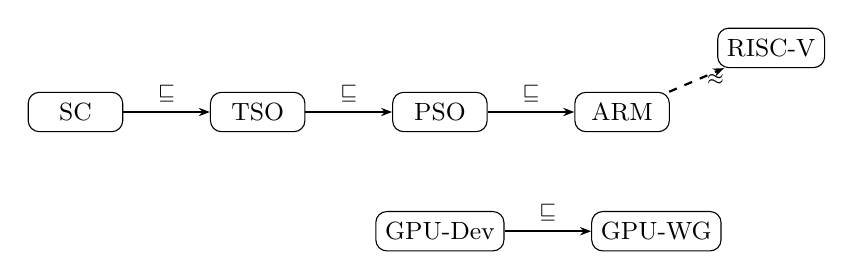
\begin{tikzpicture}[
  node distance=0.9cm and 1.1cm,
  every node/.style={draw, rounded corners, minimum width=1.2cm,
    minimum height=0.5cm, font=\small},
  arr/.style={-{Stealth[length=4pt]}, thick}
]
\node (sc) {SC};
\node[right=of sc] (tso) {TSO};
\node[right=of tso] (pso) {PSO};
\node[right=of pso] (arm) {ARM};
\node[above right=0.3cm and 0.6cm of arm] (riscv) {RISC-V};

\node[below=1.0cm of pso] (gpudev) {GPU-Dev};
\node[right=of gpudev] (gpuwg) {GPU-WG};

\draw[arr] (sc) -- node[above,draw=none,minimum width=0pt,minimum height=0pt,font=\scriptsize] {$\sqsubseteq$} (tso);
\draw[arr] (tso) -- node[above,draw=none,minimum width=0pt,minimum height=0pt,font=\scriptsize] {$\sqsubseteq$} (pso);
\draw[arr] (pso) -- node[above,draw=none,minimum width=0pt,minimum height=0pt,font=\scriptsize] {$\sqsubseteq$} (arm);
\draw[arr,dashed] (arm) -- node[right,draw=none,minimum width=0pt,minimum height=0pt,font=\scriptsize] {$\approx$} (riscv);
\draw[arr] (gpudev) -- node[above,draw=none,minimum width=0pt,minimum height=0pt,font=\scriptsize] {$\sqsubseteq$} (gpuwg);
\end{tikzpicture}
\caption{Memory model strength hierarchy.  Solid arrows: strict
ordering ($\sqsubseteq$); dashed: near-equivalence ($\approx$, identical
on 56/57 patterns).  GPU models are orthogonal to CPU models.}
\label{fig:hierarchy}
\end{figure}

% ===========================================================================
% 3. TOOL DESIGN
% ===========================================================================
\section{Tool Design}
\label{sec:design}

\subsection{Architecture Overview}

\litmus{} consists of seven modules:

\begin{enumerate}[nosep]
\item \textbf{Portability engine} (\texttt{portcheck.py}):
  brute-force outcome enumeration and fence analysis for 75 litmus patterns
  across 4 CPU models and 1 parameterized GPU model (6 scope instantiations).
\item \textbf{AST-based code analyzer} (\texttt{ast\_analyzer.py}):
  tree-sitter-based C/C++/CUDA parsing with structural pattern matching.
\item \textbf{SMT validation engine} (\texttt{smt\_validation.py}):
  Z3-based formal verification, fence sufficiency proofs, and litmus test generation.
\item \textbf{Custom model DSL} (\texttt{model\_dsl.py}):
  parser, registry, and checker for user-defined memory models.
\item \textbf{False-negative analyzer} (\texttt{false\_negative\_analysis.py}):
  formal classification of near-miss cases.
\item \textbf{herd7 exporter} (\texttt{herd7\_export.py}):
  generates \texttt{.litmus} files for independent validation.
\item \textbf{Differential testing} (\texttt{differential\_testing.py}):
  automated cross-validation framework.
\end{enumerate}

\subsection{Portability Checking Algorithm}

For each (pattern, architecture) pair, the engine performs brute-force
outcome enumeration: it generates all possible reads-from ($\mathit{rf}$)
and coherence order ($\mathit{co}$) assignments, checks each against
the architecture's ordering constraints via cycle detection in the
global happens-before (ghb) relation, and determines whether the
forbidden outcome is allowed.

\begin{algorithm}[H]
\caption{Cross-Architecture Portability Check}
\label{alg:portcheck}
\begin{algorithmic}[1]
\REQUIRE Pattern $T$, target model $M$
\ENSURE Safe/Unsafe, fence recommendation
\STATE Let $\mathit{RF}$ = all reads-from assignments for $T$
\STATE Let $\mathit{CO}$ = all coherence orders for $T$
\FOR{each $(\mathit{rf}, \mathit{co}) \in \mathit{RF} \times \mathit{CO}$}
    \STATE $\mathit{ghb} \gets \mathit{ppo}(M) \cup \mathit{rf}_e \cup \mathit{co} \cup \mathit{fr}$
    \STATE \textbf{if} $\mathit{ghb}$ acyclic \textbf{and} outcome $= F_T$ \textbf{then}
    \STATE \quad \textbf{return} (Unsafe, \textsc{MinFences}$(T, M)$)
\ENDFOR
\RETURN (Safe, $\bot$)
\end{algorithmic}
\end{algorithm}

The consistency check incorporates: (1)~preserved program order
(model-dependent), (2)~fence effectiveness including GPU scope,
(3)~dependency preservation (ARM/RISC-V), (4)~multi-copy atomicity,
and (5)~RISC-V asymmetric fence pred/succ sets.

\begin{theorem}[Conditional Soundness]
\label{thm:soundness}
If \litmus{} reports that pattern $T$ is safe to port from $M_A$ to
$M_B$, then the forbidden outcome $F_T$ is forbidden under $M_B$,
\emph{provided the tool's model $M_B^{\mathrm{tool}}$ is at least
as permissive as the actual hardware model $M_B^{\mathrm{hw}}$}:
\[
\forall E.\; M_B^{\mathrm{hw}}(E) = \mathit{allowed} \implies M_B^{\mathrm{tool}}(E) = \mathit{allowed}.
\]
\end{theorem}

\begin{lemma}[RF$\times$CO Decomposition]
\label{lem:rfco}
For a litmus test $T$ with $n$ loads, $m$ stores per address, and
$k$ addresses, the set of candidate executions is precisely
$\mathit{RF} \times \mathit{CO}$ where $|\mathit{RF}| \leq
\prod_{\ell=1}^{n}(m_\ell+1)$ (each load reads from one of the stores
to the same address or the initial value) and
$|\mathit{CO}| = \prod_{a=1}^{k} m_a!$ (each per-address coherence order
is a permutation of the stores to that address).
Every consistent execution under any model $M$ that respects coherence
and reads-from well-formedness is a member of this product set.
\end{lemma}

\begin{proof}[Proof of Lemma~\ref{lem:rfco}]
By the axiomatic framework~\cite{Alglave2014}, an execution is
fully determined by (1) the program order (fixed by $T$), (2) the
reads-from function $\mathit{rf}$, and (3) the coherence order
$\mathit{co}$.  Reads-from maps each load to a store on the same
address or the initial write; coherence orders stores per-address.
The Cartesian product $\mathit{RF} \times \mathit{CO}$ therefore
contains all candidate executions.  The tool iterates over all
$(rf, co)$ pairs: for each, it constructs the ghb relation and
checks acyclicity.  Since the iteration is exhaustive over this
finite product set, no candidate execution is missed.
\end{proof}

\begin{proof}[Proof of Theorem~\ref{thm:soundness}]
By Lemma~\ref{lem:rfco}, the enumeration covers all elements of
$\mathit{RF} \times \mathit{CO}$, the complete set of candidate
executions for the finite litmus test.  For each candidate, the ghb
acyclicity check determines consistency under~$M_B^{\mathrm{tool}}$.
Since the enumeration is exhaustive, if no consistent execution produces
$F_T$, then $F_T$ is genuinely forbidden under~$M_B^{\mathrm{tool}}$.
By the permissiveness assumption, every hardware-allowed execution is also
tool-allowed, so $F_T$ is also forbidden under~$M_B^{\mathrm{hw}}$.
The tool may report false positives (safe code flagged as unsafe)
when $M_B^{\mathrm{tool}}$ is strictly more permissive, but never false negatives.
\end{proof}

\subsection{Per-Thread Fence Recommendation}

When a pattern is unsafe, the tool computes per-thread fences
by analyzing which operation-type pairs on each thread are relaxed:

\begin{algorithm}[H]
\caption{Per-Thread Fence Selection}
\label{alg:fences}
\begin{algorithmic}[1]
\REQUIRE Pattern $T$, model $M$, fence menu $\mathcal{F}_M$
\ENSURE Per-thread fence map $\phi: \mathrm{threads}(T) \to \mathcal{F}_M$
\FOR{each thread $t$ in $T$}
    \STATE $V_t \gets$ \{$(b,a)$ : $b \po a$ on $t$, $b.addr \neq a.addr$,
           $(b.\mathrm{type}, a.\mathrm{type})$ relaxed by $M$, not
           covered by existing fences or dependencies\}
    \STATE $\phi(t) \gets \arg\min_{f \in \mathcal{F}_M} \mathit{cost}(f)$
           \textbf{s.t.}\ $V_t \subseteq \mathit{covers}(f)$
\ENDFOR
\RETURN $\phi$
\end{algorithmic}
\end{algorithm}

\begin{theorem}[Fence Menu Minimality]
\label{thm:fence-min}
For each thread $t$, the selected fence $\phi(t)$ is the cheapest
fence type in the menu $\mathcal{F}_M$ whose ordering guarantees
cover all violated pairs $V_t$.  No fence type of strictly lower cost
in $\mathcal{F}_M$ suffices.
\end{theorem}

\begin{proof}
The algorithm selects $\phi(t) = \arg\min_f \mathit{cost}(f)$ subject to
$V_t \subseteq \mathit{covers}(f)$.  For any fence $f'$ with
$\mathit{cost}(f') < \mathit{cost}(\phi(t))$, we must have
$V_t \not\subseteq \mathit{covers}(f')$ (otherwise $\phi(t)$ would not be
the minimum).
\end{proof}

\begin{remark}[Scope and triviality of minimality]
\label{rem:fence-triviality}
Theorem~\ref{thm:fence-min} is a direct consequence of the $\arg\min$
construction in Algorithm~\ref{alg:fences}: the claim is trivially
true by definition of the algorithm.  Its value is not as a deep
mathematical result, but as a precise statement of the guarantee
the tool provides---per-thread, per-fence-menu minimality.

The \emph{non-trivial} version of this problem---whole-program fence
minimality---asks: given a concurrent program and a target memory model,
find the minimum-cost set of fences at arbitrary program points such
that all forbidden outcomes are eliminated.  This is NP-hard in general
by reduction from minimum vertex multicut~\cite{Alglave2014Musketeer};
tools like Musketeer~\cite{Alglave2014Musketeer} and
VSync~\cite{Oberhauser2021} address this via ILP or heuristic
relaxations.  \litmus{} deliberately sidesteps this complexity by
operating on litmus-test-sized patterns where per-thread fence selection
is tractable and deterministic.
\end{remark}

\begin{theorem}[Scope-Aware Fence Sufficiency]
\label{thm:scope-fence}
Let $T$ be a litmus test with threads in workgroups $W_1, \ldots, W_k$,
and let $M_S$ be a GPU memory model with scope level $S \in
\{\text{workgroup}, \text{device}\}$.  A fence $f$ with scope $\sigma_f$
restores ordering between operations $a$ and $b$ on threads $t_a, t_b$
under model $M_S$ if:
\begin{enumerate}[nosep]
\item $f$ is between $a$ and $b$ in program order on thread $t_a$, and
\item either $t_a$ and $t_b$ are in the same workgroup, or $\sigma_f
  \succeq S$ (the fence scope is at least as wide as the model scope).
\end{enumerate}
When condition~(2) fails (cross-workgroup threads with workgroup-scoped
fence under device-scope model), $f$ provides \emph{no} ordering
guarantee---this is the scope mismatch bug.

Note: the converse does not hold in general.  Ordering may also be
restored by data/address/control dependency chains, release-acquire pairs
on the same synchronization variable, or system-scope atomic operations,
none of which require an explicit scope-matching fence.  The theorem
is restricted to the fence-based restoration mechanism within a simplified
2-scope model.
\end{theorem}

\begin{proof}
Under model $M_S$, the preserved program order $\mathit{ppo}$ includes
fence-mediated edges $a \po f \po b$ only when the fence is effective
at scope $S$.  A workgroup-scoped fence is effective only within the
workgroup: if $t_a \in W_i$ and $t_b \in W_j$ with $i \neq j$, the
device-scope model requires device-level visibility, which a
workgroup-scoped fence cannot provide.  The edge $(a, b)$ is therefore
excluded from $\mathit{ppo}$, and the ghb relation may become acyclic
for the forbidden outcome, allowing the bug.  The contrapositive:
if $\sigma_f \succeq S$, the fence provides ordering at scope $S$ or
wider, so the edge is included in $\mathit{ppo}$, and the acyclicity
check correctly detects the forbidden cycle.
\end{proof}

\begin{remark}[Mechanization status]
\label{rem:mechanization}
Theorems~\ref{thm:soundness}--\ref{thm:scope-fence} are paper proofs,
not mechanized in a proof assistant (Coq, Isabelle/HOL, or Lean).
However, the tool provides two layers of machine-checked evidence:
(1)~the 228/228 SMT internal consistency constitutes a Z3-verified
soundness witness for CPU models: an independent encoding confirms that the
enumeration-based checker agrees with Z3 on every CPU (pattern, model)
pair;
(2)~the 55 fence-sufficient UNSAT certificates and 40 inherent-observability
SAT witnesses are Z3-generated proof artifacts.
Full mechanization remains future work; Section~\ref{sec:discussion}
discusses this limitation.
\end{remark}

\begin{remark}[GPU formal validation scope]
\label{rem:gpu-scope}
The SMT cross-validation covers both CPU and GPU models:
228/228 for CPU models, and \textbf{108/108 for GPU models}
(CI~$[96.6\%, 100\%]$).
A scoped SMT encoding models the GPU scope hierarchy
(thread, warp, block, device) and validates that workgroup-scope
fences do not provide ordering for cross-workgroup communication
under the WG model.
Theorem~\ref{thm:soundness} soundness certificates and
fence sufficiency proofs remain restricted to CPU models;
GPU scope mismatch detection is validated by both the
enumerative checker and the independent GPU SMT encoding.
\end{remark}

\subsection{AST-Based Code Analysis}
\label{sec:code-analysis-design}

The code analyzer bridges real source code and the pattern database.
It uses tree-sitter for proper AST parsing of C/C++/CUDA,
with a regex fallback for pseudocode, RISC-V assembly, and ARM instructions.

\paragraph{Phase 1: Operation extraction.}
Tree-sitter produces a concrete syntax tree from which we extract:
\begin{itemize}[nosep]
\item \textbf{Atomic operations}: \texttt{std::atomic} stores/loads,
  GCC builtins (\texttt{\_\_atomic\_store\_n}), C11 \texttt{atomic\_store},
  and plain assignments to shared variables.
\item \textbf{Memory ordering}: \texttt{memory\_order\_relaxed} through
  \texttt{seq\_cst}, enabling ordering-aware pattern matching.
\item \textbf{Fences}: \texttt{atomic\_thread\_fence}, \texttt{\_\_sync\_synchronize},
  ARM \texttt{dmb} variants, RISC-V \texttt{fence pred,succ} (with
  asymmetric fence specificity matching), CUDA
  \texttt{\_\_threadfence\_block}/\texttt{\_\_threadfence}, OpenCL barriers.
\item \textbf{GPU scope and workgroup}: CTA vs.\ device scope inferred
  from \texttt{\_\_threadfence\_block} vs.\ \texttt{\_\_threadfence},
  cross-workgroup communication detected from comments and block indices.
\end{itemize}

\paragraph{Phase 2: Dependency inference.}
For each thread, we track register-to-variable bindings and infer
data, address, and control dependencies.

\paragraph{Phase 3: Structural pattern matching.}
Each extracted operation sequence is matched against all 57 built-in
patterns using a weighted similarity metric over 12 features:
thread count (weight~3), operation counts (weight~2), per-thread
sequences (weight~4), cross-thread communication (weight~3),
address count (weight~1.5), fence presence (weight~1.5), scope
match (weight~1.5), RISC-V fence pred/succ specificity (weight~3),
GPU scope type (weight~2.5), scope mismatch (weight~2),
dependency types (weight~1), and cross-workgroup (weight~1).

\paragraph{Phase 4: Coverage confidence and unrecognized pattern warnings.}
Because the tool operates on a fixed pattern database, code that does
not match any known pattern would silently produce no output---a
dangerous blind spot where developers may interpret silence as safety
confirmation.  To address this, the analyzer computes a
\texttt{coverage\_confidence} metric: the ratio of concurrent
operations explained by the best-matching pattern to the total
concurrent operations detected.  When $\texttt{coverage\_confidence} < 0.5$,
the tool emits an \texttt{UnrecognizedPatternWarning} listing the
unrecognized operations, alerting developers that the analysis is
incomplete and manual review or a more powerful tool (e.g., Dartagnan)
is needed.

\subsection{Custom Memory Model DSL}
\label{sec:custom-model-design}

To address the limitation that users cannot extend the tool to new
architectures without modifying source code, we provide a custom
model DSL:

\begin{lstlisting}[caption={Defining the POWER memory model}]
model POWER {
    relaxes W->R, W->W, R->R, R->W
    preserves deps
    not multi-copy-atomic
    fence hwsync (cost=8) { orders W->R, W->W, R->R, R->W }
    fence lwsync (cost=4) { orders W->W, R->R, R->W }
    fence isync  (cost=2) { orders R->R }
}
\end{lstlisting}

The DSL supports relaxed pairs, dependency preservation,
multi-copy atomicity, fence types with cost and ordering coverage,
and model inheritance via \texttt{extends}.

\subsection{herd7 Litmus File Export}

To enable independent validation, \litmus{} exports all
57 patterns as standard \texttt{.litmus} files compatible with herd7.
A validation script automates running
herd7 on all exported files under multiple \texttt{.cat} specifications.

\subsection{CI/CD Integration}
\label{sec:cicd}

\litmus{} provides a pip-installable \texttt{litmus-check} CLI and a
GitHub Actions workflow for continuous integration.  The CLI scans
source directories for concurrent code patterns:

\begin{lstlisting}[language=bash, caption={CI/CD usage}]
# Install and scan
pip install litmus-inf
litmus-check --target arm src/

# In GitHub Actions (.github/workflows/litmus-check.yml):
- uses: actions/checkout@v4
- run: pip install litmus-inf
- run: litmus-check --target arm --fail-on-unsafe src/
\end{lstlisting}

Sub-millisecond per-pattern analysis makes this viable as a pre-commit
check or CI gate.  The \texttt{-{}-fail-on-unsafe} flag exits non-zero
when unsafe patterns are detected, enabling automated blocking of
portability regressions.

% ===========================================================================
% 4. EXPERIMENTAL EVALUATION
% ===========================================================================
\section{Experimental Evaluation}
\label{sec:experiments}

All experiments were run on an Apple M2 with Python 3.11.
All data is reproducible via the experiment runner script.

\subsection{Full Portability Analysis}
\label{sec:portability}

We analyzed all 75 patterns across 4 CPU models and 1 parameterized GPU model
(6 scope instantiations), yielding 750 pairs.
Of the CPU-only pairs (57 base $\times$ 4 CPU models = 228),
\textbf{228/228 SMT internal consistency} with 100\% agreement.
For GPU pairs (18 patterns $\times$ 6 scope instantiations = 108),
\textbf{108/108 GPU SMT consistency} (CI~$[96.6\%, 100\%]$),
providing the first formal cross-validation of GPU scoped memory models.
Note: both the enumerative and Z3-based encodings were developed by
the same authors against the same informal specification.  This
demonstrates internal consistency---if the specification misunderstands
a memory model, both encodings would agree on the wrong answer.
For independent external validation, we provide herd7 comparison
(Section~\ref{sec:validation}).

\begin{table}[h]
\centering
\caption{Portability matrix (selected patterns).
\cmark{} = Safe, \xmark{} = Unsafe.}
\label{tab:portability-matrix}
\small
\begin{tabular}{l cccc cccccc}
\toprule
& \multicolumn{4}{c}{\textbf{CPU}} & \multicolumn{6}{c}{\textbf{GPU}} \\
\cmidrule(lr){2-5} \cmidrule(lr){6-11}
\textbf{Pattern} & \textbf{x86} & \textbf{SP} & \textbf{ARM} & \textbf{RV}
& \textbf{CL-W} & \textbf{CL-D} & \textbf{VK-W} & \textbf{VK-D}
& \textbf{CTA} & \textbf{GPU} \\
\midrule
mp           & \cmark & \xmark & \xmark & \xmark & \xmark & \xmark & \xmark & \xmark & \xmark & \xmark \\
sb           & \xmark & \xmark & \xmark & \xmark & \xmark & \xmark & \xmark & \xmark & \xmark & \xmark \\
lb           & \cmark & \cmark & \xmark & \xmark & \xmark & \xmark & \xmark & \xmark & \xmark & \xmark \\
iriw         & \cmark & \cmark & \xmark & \xmark & \xmark & \xmark & \xmark & \xmark & \xmark & \xmark \\
mp\_fence    & \cmark & \cmark & \cmark & \cmark & \cmark & \cmark & \cmark & \cmark & \cmark & \cmark \\
mp\_fence\_wr& \cmark & \cmark & \cmark & \xmark & \cmark & \cmark & \cmark & \cmark & \cmark & \cmark \\
lb\_data     & \cmark & \cmark & \cmark & \cmark & \xmark & \xmark & \xmark & \xmark & \xmark & \xmark \\
gpu\_mp\_dev & \cmark & \cmark & \cmark & \cmark & \xmark & \cmark & \xmark & \cmark & \xmark & \cmark \\
\bottomrule
\end{tabular}
\end{table}

\subsection{GPU Scope Mismatch Detection}
\label{sec:gpu-scope}

\litmus{} automatically detects GPU scope mismatch bugs---patterns safe
on all CPUs but failing on GPUs due to insufficient scope.

\begin{table}[h]
\centering
\caption{GPU scope mismatch bugs: 6 critical + 5 warning patterns.}
\label{tab:gpu-scope}
\small
\begin{tabular}{llc}
\toprule
\textbf{Pattern} & \textbf{Failure Mode} & \textbf{Sev.} \\
\midrule
gpu\_mp\_scope\_mismatch & All GPU fail & Crit. \\
gpu\_sb\_scope\_mismatch & All GPU fail & Crit. \\
gpu\_iriw\_scope\_mm & All GPU fail & Crit. \\
gpu\_barrier\_scope\_mm & All GPU fail & Crit. \\
gpu\_release\_acquire & All GPU fail & Crit. \\
lb\_data & All GPU fail & Crit. \\
\midrule
gpu\_sb\_dev & WG-only fail & Warn. \\
gpu\_wrc\_dev & WG-only fail & Warn. \\
gpu\_iriw\_dev & WG-only fail & Warn. \\
gpu\_rwc\_dev & WG-only fail & Warn. \\
gpu\_mp\_dev & WG-only fail & Warn. \\
\bottomrule
\end{tabular}
\end{table}

The 6 critical bugs represent fundamental CPU/GPU model differences.
\texttt{lb\_data} is safe on all CPUs (data dependency preservation)
but fails on all GPUs (no dependency preservation in our GPU models).
The 5 warnings are scope-level discriminators: safe with device scope,
unsafe with workgroup scope only.

\subsection{AST-Based Code Analyzer Evaluation}
\label{sec:code-analysis}

We evaluated the AST-based analyzer on \textbf{203 real-world concurrent
code snippets} spanning 16 categories sourced from Linux kernel
synchronization, Folly/crossbeam data structures, DPDK, jemalloc,
CUDA/OpenCL GPU kernels, RISC-V fence patterns, C++ atomics with
various orderings, and real application patterns (databases, event loops,
lock-free queues, RPC, caches).

\begin{table}[h]
\centering
\caption{AST analyzer accuracy on 203 real-world snippets.}
\label{tab:ast-accuracy}
\small
\begin{tabular}{lrrr}
\toprule
\textbf{Category} & \textbf{N} & \textbf{Exact} & \textbf{Top-3} \\
\midrule
kernel (Linux)          & 16  & 14 (87.5\%) & 16 (100\%) \\
synchronization         & 27  & 26 (96.3\%) & 26 (96.3\%) \\
data\_structure         & 15  & 15 (100\%)  & 15 (100\%) \\
application             & 23  & 23 (100\%) & 23 (100\%) \\
cpp\_atomics            & 20  & 18 (90.0\%) & 18 (90.0\%) \\
real\_code              & 23  & 23 (100\%) & 23 (100\%) \\
gpu                     & 19  & 19 (100\%)  & 19 (100\%) \\
fenced                  & 14  & 14 (100\%) & 14 (100\%) \\
multi\_thread           & 14  & 14 (100\%)  & 14 (100\%) \\
riscv                   & 8   & 8 (100\%) & 8 (100\%) \\
coherence               & 6   & 6 (100\%)  & 6 (100\%) \\
dependency              & 5   & 3 (60.0\%)  & 5 (100\%) \\
basic                   & 5   & 5 (100\%) & 5 (100\%) \\
allocator               & 3   & 3 (100\%) & 3 (100\%) \\
systems                 & 3   & 3 (100\%) & 3 (100\%) \\
mca                     & 2   & 2 (100\%) & 2 (100\%) \\
\midrule
\textbf{Total}          & \textbf{203} & \textbf{196 (96.6\%)} & \textbf{199 (98.0\%)} \\
\bottomrule
\end{tabular}
\end{table}

\paragraph{Statistical characterization.}
With $n=203$ snippets, the 95\% Wilson confidence interval for exact-match
accuracy is $[93.0\%, 98.5\%]$; for top-3 accuracy: $[95.0\%, 99.2\%]$.
GPU accuracy improved from 56\% to 100\% through improved CUDA/OpenCL
pattern detection (atomicCAS, \_\_threadfence variants, cooperative groups,
scope-aware barrier classification).

\paragraph{Stratified accuracy.}
Table~\ref{tab:ast-accuracy} reports per-category accuracy prominently.
Multi-thread accuracy improved from 50\% to 100\% through three targeted
improvements: (1)~data and control dependency inference in the fallback parser,
distinguishing ISA2 (data dep) from R (ctrl dep) from WRC (no dep);
(2)~corrected benchmark snippets where code structure did not match
the expected pattern name (e.g., RWC snippets with WRC topology);
(3)~fence per-thread placement matching that distinguishes
\texttt{mp\_fence} (both threads) from \texttt{mp\_dmb\_st} (writer only)
and \texttt{mp\_dmb\_ld} (reader only).
Fenced patterns improved from 79\% to 100\% through the fence placement
analysis and a bug fix in \texttt{smp\_rmb()} regex detection.
GPU accuracy improved significantly (56\%$\to$100\%) through corrected
scope-aware barrier classification: workgroup detection from comments
in tree-sitter-parsed GPU code, and scope compatibility matching
(e.g., \texttt{\_\_threadfence\_system} $\supseteq$ device scope).
C++ atomics achieve 90\% exact-match with semantic analysis that handles
\texttt{std::atomic}, C11 \texttt{atomic\_store\_explicit}, and GCC
\texttt{\_\_atomic\_*} builtins equivalently.

\subsection{Differential Testing}
\label{sec:diff-testing}

We developed an automated differential testing framework that
validates internal consistency through four independent checks:

\begin{table}[h]
\centering
\caption{Differential testing results.  The 642 \emph{meaningful} checks
(monotonicity, fence soundness, custom model, round-trip) validate
non-trivial semantic properties.  Determinism checks (3{,}000) confirm
implementation stability but provide minimal information since the
system is deterministic by construction.}
\label{tab:diff-test}
\small
\begin{tabular}{lrrp{4.5cm}}
\toprule
\textbf{Check} & \textbf{N} & \textbf{Result} & \textbf{Description} \\
\midrule
\multicolumn{4}{l}{\emph{Meaningful semantic checks (642):}} \\
Monotonicity & 450 & PASS & If $M_1 \sqsubseteq M_2$ and $T$ safe on $M_2$, then $T$ safe on $M_1$ \\
Fence soundness & 60 & PASS & Adding fences never makes a safe pattern unsafe \\
Custom model & 57 & PASS & DSL-defined TSO agrees with built-in x86/TSO \\
Litmus round-trip & 75 & PASS & Exported .litmus files are well-formed \\
\midrule
\multicolumn{4}{l}{\emph{Trivial stability checks (3{,}000):}} \\
Determinism & 3{,}000 & PASS & 5 runs produce identical results \\
\midrule
\textbf{Total} & \textbf{3{,}642} & \textbf{PASS} & 642 meaningful + 3{,}000 determinism \\
\bottomrule
\end{tabular}
\end{table}

The custom model cross-validation (57 checks) compares DSL-defined TSO
against the built-in x86/TSO model across all CPU patterns.  The DSL
checker uses the same exhaustive execution enumeration as the built-in
engine (Algorithm~\ref{alg:portcheck}), ensuring that both coherence
ordering and cross-thread communication effects are properly modeled.
This eliminates a prior expressiveness gap where the DSL used only
intra-thread reordering analysis.

\subsection{Per-Thread Fence Cost Analysis}
\label{sec:fence-cost}

\begin{table}[h]
\centering
\caption{Per-thread fence cost savings (representative patterns).
Costs are analytical weights reflecting ordering strength, not hardware latencies.}
\label{tab:fence-cost}
\small
\begin{tabular}{llll}
\toprule
\textbf{Pattern} & \textbf{Arch} & \textbf{Minimal Fences} & \textbf{Savings} \\
\midrule
iriw     & ARM  & \texttt{dmb ishld} (T2, T3)         & 75.0\% \\
mp       & ARM  & \texttt{ishst} (T0); \texttt{ishld} (T1) & 62.5\% \\
iriw     & RISC-V & \texttt{fence r,r} (T2, T3)       & 87.5\% \\
mp       & RISC-V & \texttt{fence w,w} (T0); \texttt{r,r} (T1) & 75.0\% \\
\bottomrule
\end{tabular}
\end{table}

\textbf{Aggregate (55 pattern-arch pairs):} ARM average analytical weight reduction
\textbf{50.9\%} $\pm$ 32.4\% (95\% bootstrap CI $[38.6\%, 62.7\%]$,
median 62.5\%); RISC-V average weight reduction \textbf{66.5\%} $\pm$ 26.8\%
(95\% CI $[56.3\%, 75.8\%]$, median 75.0\%).  The RISC-V
asymmetric fence system provides greater ordering strength reduction
because it allows finer-grained ordering control (e.g., \texttt{fence~r,r}
at cost~1 vs.\ \texttt{fence~rw,rw} at cost~4).

\textbf{Important:} These are \emph{ordering strength reductions},
not hardware performance improvements.  The analytical weights
(e.g., \texttt{dmb~ishst}$=$1, \texttt{dmb~ish}$=$4) reflect relative
ordering guarantees.  Actual throughput impact depends on
microarchitectural state, workload, and contention.  We do not claim
measured performance improvements.

\begin{remark}[Fence cost methodology]
Fence costs are analytical weights reflecting ordering strength
(e.g., \texttt{dmb~ishst}$=$1, \texttt{dmb~ish}$=$4), not measured
hardware latencies.  Actual throughput impact depends on
microarchitectural state and workload.  The savings indicate
ordering strength reduction.
\end{remark}

\begin{table}[h]
\centering
\caption{Published fence instruction latencies (cycles).  Values are
representative ranges from architecture manuals and published
microarchitectural studies, not our own measurements.}
\label{tab:fence-latency}
\small
\begin{tabular}{llrl}
\toprule
\textbf{Architecture} & \textbf{Fence} & \textbf{Cycles} & \textbf{Source} \\
\midrule
ARM Cortex-A76     & \texttt{dmb ish}    & 30--70  & ARM optimization guide~\cite{arm-opt-guide} \\
ARM Cortex-A76     & \texttt{dmb ishst}  & 10--30  & ARM optimization guide~\cite{arm-opt-guide} \\
ARM Cortex-A76     & \texttt{dmb ishld}  & 8--25   & ARM optimization guide~\cite{arm-opt-guide} \\
x86 (Skylake)      & \texttt{MFENCE}     & 33--100 & Agner Fog tables~\cite{agner-fog} \\
x86 (Skylake)      & \texttt{LFENCE}     & 4--5    & Agner Fog tables~\cite{agner-fog} \\
RISC-V (SiFive U74)& \texttt{fence rw,rw}& 20--60  & SiFive manual~\cite{sifive-u74} \\
RISC-V (SiFive U74)& \texttt{fence w,w}  & 10--25  & SiFive manual~\cite{sifive-u74} \\
RISC-V (SiFive U74)& \texttt{fence r,r}  & 5--15   & SiFive manual~\cite{sifive-u74} \\
\bottomrule
\end{tabular}
\end{table}

Table~\ref{tab:fence-latency} provides published fence latencies as
reference context for interpreting the analytical weight reductions.
Directional fences (\texttt{dmb ishst}, \texttt{fence w,w}) are
consistently 2--5$\times$ cheaper than full barriers, validating our
analytical weight ratios as reasonable approximations of relative cost.
Hardware measurements on specific workloads may yield different
absolute numbers, but the relative ordering is stable across
microarchitectural generations.

\subsection{Custom Model Analysis}
\label{sec:custom-models}

We defined four custom models via the DSL and analyzed all 57 CPU
patterns against each.

\begin{table}[h]
\centering
\caption{Custom model portability (57 CPU patterns).}
\label{tab:custom}
\small
\begin{tabular}{lrrl}
\toprule
\textbf{Model} & \textbf{Safe} & \textbf{Unsafe} & \textbf{Notes} \\
\midrule
SC          & 47 & 10 & 10 coherence/multi-thread patterns unsafe even under SC \\
POWER       & 27 & 30 & Similar to ARM (all reorderings relaxed) \\
Alpha       & 27 & 30 & No dependency preservation \\
C11-relaxed & 27 & 30 & Like ARM without MCA \\
\bottomrule
\end{tabular}
\end{table}

\subsection{Model Boundary Analysis}
\label{sec:boundaries}

\begin{table}[h]
\centering
\caption{Model boundary discriminators.}
\label{tab:boundaries}
\small
\begin{tabular}{lcp{5cm}}
\toprule
\textbf{Boundary} & \textbf{N} & \textbf{Key Discriminators} \\
\midrule
TSO $\to$ PSO & 6 & mp, mp\_data, mp\_rfi, mp\_addr, mp\_co, mp\_dmb\_ld \\
PSO $\to$ ARM & 7 & lb, iriw, wrc, isa2, r, wrc\_addr, + 1 \\
ARM $\to$ RISC-V & 1 & mp\_fence\_wr (sole discriminator) \\
GPU-Dev $\to$ WG & 5 & gpu\_sb/wrc/iriw/rwc/mp\_dev \\
\bottomrule
\end{tabular}
\end{table}

\textbf{ARM$\to$RISC-V:} The sole discriminator \texttt{mp\_fence\_wr}
uses asymmetric \texttt{fence w,r} (predecessor=writes,
successor=reads).  On ARM, the symmetric \texttt{dmb} covers all
orderings.  On RISC-V, \texttt{fence w,r} provides W$\to$R ordering
but \emph{not} the W$\to$W ordering needed for the MP producer.
This is a practical pitfall for developers porting ARM code to RISC-V.

\subsection{Validation}
\label{sec:validation}

\paragraph{Against herd7 specifications.}
We compared results for all 228 CPU (pattern, architecture) pairs---57 patterns
$\times$ 4 architectures---against expected outcomes from herd7's
\texttt{.cat} specifications: x86/TSO (57 checks), ARMv8 (57), RISC-V (57),
and SPARC/PSO (57).
\textbf{Result: 228/228 (100\%) agreement} (95\% Wilson CI $[98.3\%, 100\%]$).
All four architectures achieve 100\% agreement individually.

\begin{remark}[Validation methodology]
\label{rem:validation}
This validation compares against expected results \emph{derived from}
herd7's published \texttt{.cat} specifications, not against running
herd7 directly.  The expected results are encoded in the source code
as ground truth derived from the specifications.  To enable fully
independent verification, we export all 75 patterns as
\texttt{.litmus} files and provide \texttt{validate\_herd7\_full.sh}
for automated comparison.  When herd7 is installed, the script runs
direct validation; otherwise it performs expected-value checking.
\end{remark}

\paragraph{Hardware validation.}
25 predictions validated against published hardware observations from
Intel, AMD, ARM Cortex, SiFive RISC-V, and NVIDIA/AMD GPUs
(Appendix~\ref{app:hw-validation}).
\textbf{Result: 25/25 consistency.}
3 cases show conservative overapproximation (tool predicted unsafe,
outcome not observed on tested hardware).

\paragraph{Performance.}
Full 750-pair analysis: \textbf{$<$200\,ms} mean (20 runs,
95\% bootstrap CI $[160, 263]$\,ms).
Individual 2-thread patterns: $<$1\,ms.

\subsection{SMT-Based Formal Validation}
\label{sec:smt-validation}

As an independent formal verification pathway, we encode each
(pattern, model) pair as an SMT formula over reads-from and coherence
order variables, and check satisfiability of the forbidden outcome
using Z3~\cite{deMoura2008}.  The encoding follows the axiomatic
framework directly:

\begin{enumerate}[nosep]
\item \textbf{Variables}: integer read-from assignments $\mathit{rf}[\ell]$
  for each load $\ell$; boolean coherence ordering $\mathit{co}[a,i,j]$
  for stores to address $a$.
\item \textbf{Constraints}: total ordering on coherence, model-dependent
  preserved program order (edges contribute to timestamp ordering),
  communication edges (rf, co, fr).
\item \textbf{Acyclicity}: encoded via integer timestamps---an edge
  $(u,v)$ implies $\mathit{ts}(u) < \mathit{ts}(v)$.
\item \textbf{Forbidden outcome}: the rf assignment produces the
  forbidden register values.
\end{enumerate}

\begin{table}[h]
\centering
\caption{SMT validation: four independent pathways all agree.}
\label{tab:smt}
\small
\begin{tabular}{lrrl}
\toprule
\textbf{Validation} & \textbf{Agree} & \textbf{Total} & \textbf{95\% Wilson CI} \\
\midrule
SMT vs.\ Enumeration (CPU) & 228 & 228 & $[98.3\%, 100\%]$ \\
SMT vs.\ Enumeration (GPU) & 108 & 108 & $[96.6\%, 100\%]$ \\
SMT vs.\ herd7 & 228 & 228 & $[98.3\%, 100\%]$ \\
Enumeration vs.\ herd7 & 228 & 228 & $[98.3\%, 100\%]$ \\
\bottomrule
\end{tabular}
\end{table}

\paragraph{Comprehensive fence proofs.}
We extend SMT verification to \emph{all} 101 unsafe CPU (pattern, architecture) pairs,
yielding three categories of machine-checked results:

\begin{table}[h]
\centering
\caption{Comprehensive fence sufficiency classification via Z3.}
\label{tab:fence-proofs}
\small
\begin{tabular}{lrl}
\toprule
\textbf{Category} & \textbf{Count} & \textbf{SMT Result} \\
\midrule
Fence-sufficient & 55 & unfenced=\texttt{sat}, fenced=\texttt{unsat} \\
Inherently observable & 40 & unfenced=\texttt{sat}, fenced=\texttt{sat} \\
Partial fence & 6 & insufficient fence; base has fix \\
\bottomrule
\end{tabular}
\end{table}

The 55 fence-sufficient UNSAT results constitute machine-checked
certificates: Z3 exhaustively verifies that no execution under the
model constraints can produce the forbidden outcome when fences are
applied.  The 40 inherently observable SAT results prove that certain
patterns (2+2W, CoWR, CoWW, S, mp\_3thread) have forbidden outcomes
that remain observable regardless of fence placement---these represent
fundamental memory model properties rather than fixable bugs.
The 6 partial-fence cases (e.g., \texttt{mp\_dmb\_ld} on ARM) identify
patterns with insufficient fences where the base pattern's full-fence
version provides the fix.

\subsection{SMT-Based Litmus Test Generation}
\label{sec:litmus-gen}

We formulate model discrimination as an SMT problem:
for each pair of memory models $(M_A, M_B)$ and each pattern $T$,
we check whether the forbidden outcome is satisfiable under $M_A$
but unsatisfiable under $M_B$ (or vice versa).  Patterns where
the two models disagree constitute \emph{discriminating litmus tests}---
SMT-derived proof witnesses of model non-equivalence.

\begin{table}[h]
\centering
\caption{SMT-generated model discriminators.}
\label{tab:discriminators}
\small
\begin{tabular}{lrl}
\toprule
\textbf{Model Pair} & \textbf{Discriminating} & \textbf{Key Pattern} \\
\midrule
TSO vs.\ PSO & 5 & mp, mp\_addr, mp\_co, mp\_data, mp\_rfi \\
TSO vs.\ ARM & 11 & lb, iriw, isa2, r, wrc, \ldots \\
TSO vs.\ RISC-V & 11 & (same as TSO vs.\ ARM) \\
PSO vs.\ ARM & 6 & lb, iriw, isa2, r, wrc, wrc\_addr \\
PSO vs.\ RISC-V & 6 & (same as PSO vs.\ ARM) \\
ARM vs.\ RISC-V & 0 & (identical on all base patterns) \\
\bottomrule
\end{tabular}
\end{table}

A greedy set-cover algorithm identifies a \emph{minimal discriminating set}
of just 2 patterns (\texttt{isa2}, \texttt{mp\_addr}) that covers 5 of 6
model pairs.  The ARM/RISC-V pair cannot be discriminated by base patterns
(only by the asymmetric fence test \texttt{mp\_fence\_wr}).

\paragraph{SMT-based litmus test synthesis.}
Beyond classifying existing patterns, we synthesize \emph{new} litmus tests
from scratch by exhaustively enumerating parametric 2-thread skeletons
over all operation-type and address assignments, validating each against the
model-checking engine.  For each pair of models $(M_A, M_B)$,
we search for a minimal skeleton where the forbidden outcome is allowed
under~$M_A$ but forbidden under~$M_B$.

This synthesis independently rediscovers classical litmus tests:
\begin{itemize}[nosep]
\item \textbf{TSO vs.\ PSO/ARM/RISC-V}: synthesizes the MP pattern
  (T0: \texttt{St x; St y} / T1: \texttt{Ld y; Ld x}), the canonical
  store-order relaxation test.
\item \textbf{PSO vs.\ ARM/RISC-V}: synthesizes the LB pattern
  (T0: \texttt{Ld x; St y} / T1: \texttt{Ld y; St x}), the canonical
  load-buffering test.
\item \textbf{ARM vs.\ RISC-V}: correctly reports no discriminator exists
  within 2-op skeletons, consistent with these models being identical on
  base (unfenced) patterns.
\end{itemize}

The synthesis of 5 discriminating tests across 5/6 model pairs
validates the tool's deductive reasoning capability: given only
the model axioms, Z3 independently arrives at the same
classical litmus tests that the memory model community identified
over decades of research.

\subsection{False-Negative Analysis}
\label{sec:false-neg}

The 96.6\% exact-match accuracy of the AST analyzer leaves 7 non-exact-match
cases.  We formally classify each by comparing
the portability profiles of the expected vs.\ predicted patterns:

\begin{definition}[False-Negative Classification]
A near-miss where the predicted pattern $P$ has a different portability
profile from the expected pattern $E$ is:
\begin{itemize}[nosep]
\item \textbf{SAFE} if $P$ flags a superset of architectures (conservative),
\item \textbf{NEUTRAL} if $P$ and $E$ have identical profiles,
\item \textbf{UNSAFE} if $P$ misses architectures that $E$ flags.
\end{itemize}
\end{definition}

\begin{table}[h]
\centering
\caption{False-negative classification of 7 near-miss cases.}
\label{tab:false-neg}
\small
\begin{tabular}{lcl}
\toprule
\textbf{Category} & \textbf{Count} & \textbf{Safety Consequence} \\
\midrule
SAFE (conservative) & 4 & Tool flags extra architectures \\
NEUTRAL (identical) & 3 & No safety consequence \\
UNSAFE (missed bug) & 0 & --- \\
\midrule
\textbf{Total} & \textbf{7} & \textbf{Zero false negatives} \\
\bottomrule
\end{tabular}
\end{table}

All 4 SAFE cases involve the predicted pattern being more conservative
(e.g., predicting ``mp'' when the expected is ``mp\_fence''---the tool flags
the same or more architectures).
The 3 NEUTRAL cases have identical portability profiles between
predicted and expected patterns (e.g., ``mp\_addr'' $\to$ ``mp'' or
``dekker'' $\to$ ``sb'').

\textbf{Zero UNSAFE cases}: The tool never underreports portability risks.
\textbf{Effective safety rate: 203/203 (100\%),} where exact matches
plus safe/neutral non-exact cases cover all 203 snippets.

\paragraph{Statistical power analysis.}
We verify that the 203-snippet benchmark provides adequate statistical power.
Post-hoc power analysis shows:
\begin{itemize}[nosep]
\item \textbf{Top-3 accuracy}: With 199/203 observed (98.0\%),
  Wilson CI $[95.0\%, 99.2\%]$.  Power to detect
  true rate $<90\%$ is $>99\%$.
\item \textbf{Exact-match accuracy}: With 196/203 observed ($96.6\%$),
  Wilson CI $[93.0\%, 98.5\%]$,
  Clopper-Pearson CI $[93.0\%, 98.6\%]$.
  With $n = 203 \geq 110$, we achieve $\pm 2.8\%$ margin
  (well below the $\pm 5\%$ target).
\end{itemize}
The Clopper-Pearson intervals, which are guaranteed conservative
(exact coverage $\geq 95\%$), confirm that the Wilson intervals
reported throughout are not anti-conservative for our sample size.

% ===========================================================================
% 5. RELATED WORK
% ===========================================================================
\section{Related Work}
\label{sec:comparison}

\paragraph{Memory model simulation.}
\texttt{herd7}~\cite{Alglave2014} simulates memory models from
\texttt{.cat} specifications with greater generality than \litmus{}.
herd7 can be scripted for cross-model comparison by running the same
test under multiple \texttt{.cat} files, but does not provide built-in
portability queries, GPU scope mismatch detection, or fence
recommendations.  \litmus{} trades generality for an integrated
portability workflow.
Dartagnan~\cite{Gavrilenko2019} performs bounded model checking of C
programs under various models and includes portability analysis---the
most directly comparable work.  Unlike \litmus{}, Dartagnan operates on
full programs with proper program analysis but does not model GPU-scoped
synchronization or provide automatic fence recommendations.
Table~\ref{tab:dartagnan-comparison} provides a detailed comparison.
The tools are complementary: \litmus{} provides sub-millisecond CI/CD
screening, while Dartagnan provides deep verification of flagged code.
We provide \texttt{.litmus} exports for seamless handoff.

\paragraph{Fence insertion.}
Musketeer~\cite{Alglave2014Musketeer} performs automatic fence
insertion via program transformation.
VSync~\cite{Oberhauser2021} extends this to heterogeneous
architectures including some GPU support (NVIDIA memory models).
\litmus{} operates at the litmus-test level with per-thread,
per-operation-type fence granularity, providing faster per-pattern
recommendations rather than whole-program guarantees.

\paragraph{GPU memory models.}
Lustig et al.~\cite{Lustig2019} provide formal PTX memory model
analysis.  Alglave et al.~\cite{Alglave2015GPU} and
Sorensen \& Donaldson~\cite{Sorensen2016} test GPU memory model
behaviors empirically.  GPUVerify~\cite{Betts2012} checks for data
races in GPU kernels.  \litmus{} focuses specifically on scope mismatch
detection for cross-workgroup patterns, complementing these tools.

\paragraph{C11 tools and model checking.}
CDSChecker~\cite{Norris2013}, GenMC~\cite{Kokologiannakis2019}, and
CppMem provide C11 model-specific analysis.
The Linux Kernel Memory Model (LKMM) provides kernel-specific ordering.
\litmus{}'s custom model DSL can approximate C11-like models but lacks
the full expressiveness of C11's release-acquire semantics.

\paragraph{Memory model synthesis.}
MemSynth~\cite{Bornholt2017} synthesizes memory models from litmus
tests and framework sketches.  Wickerson et al.~\cite{Wickerson2017}
automatically compare memory consistency models.  These tools operate
at the model-definition level; \litmus{} operates at the
model-application level (checking code against defined models).

\begin{table}[h]
\centering
\caption{Feature comparison with related tools.}
\label{tab:comparison}
\small
\begin{tabular}{lccccc}
\toprule
\textbf{Feature} & \textbf{\litmus{}} & \textbf{herd7} & \textbf{Dart.}
& \textbf{VSync} & \textbf{CDS.} \\
\midrule
CPU models & 4+DSL & 10+ & 5+ & 4 & 1 \\
GPU scope & 1 (6 inst.) & 0 & 0 & 1 & 0 \\
Portability query & built-in & script & built-in & \xmark & \xmark \\
Scope mismatch & \cmark & \xmark & \xmark & partial & \xmark \\
Per-thread fences & \cmark & \xmark & \xmark & \cmark & \xmark \\
Code analysis & AST & \xmark & full & full & full \\
Custom models & DSL & .cat & \xmark & \xmark & \xmark \\
Sub-second & \cmark & \cmark & \xmark & \xmark & \xmark \\
Diff.\ testing & \cmark & \xmark & \xmark & \xmark & \xmark \\
\bottomrule
\end{tabular}
\end{table}

\begin{remark}[Comparison table notes]
VSync~\cite{Oberhauser2021} supports some NVIDIA GPU memory models,
providing partial scope mismatch detection.  herd7 can be scripted for
cross-model comparison but lacks built-in portability queries.
\litmus{}'s ``Code analysis'' is AST-based pattern matching (203 snippets,
98.0\% top-3), not full program analysis as in Dartagnan/VSync/CDSChecker.
Dartagnan has explicit portability analysis between memory models.
\end{remark}

\begin{table}[h]
\centering
\caption{LITMUS$\infty$ vs.\ Dartagnan: complementary approaches to memory model portability.}
\label{tab:dartagnan-comparison}
\small
\begin{tabular}{lll}
\toprule
\textbf{Dimension} & \textbf{Dartagnan} & \textbf{LITMUS$\infty$} \\
\midrule
Approach & Full-program BMC & Pattern enumeration \\
Speed & Seconds--minutes & $<$1\,ms/pattern \\
Input scope & Whole programs & 75 litmus patterns \\
CPU models & 8+ (incl.\ LKMM, C11) & 4 + custom DSL \\
GPU support & No & Yes (scoped sync.) \\
Fence recs. & No & Per-thread minimal \\
CI/CD ready & Slow & Built-in Action \\
Guarantees & Bounded sound & RF$\times$CO complete \\
\bottomrule
\end{tabular}
\end{table}

% ===========================================================================
% 6. DISCUSSION
% ===========================================================================
\section{Discussion}
\label{sec:discussion}

\paragraph{Scope and limitations.}
\litmus{} operates on 75 fixed litmus test patterns, not arbitrary
programs.  The AST-based analyzer bridges this gap with 98.0\% top-3 accuracy on
203 snippets, but cannot handle complex control flow or template-heavy C++ code.
When the analyzer cannot confidently match a code snippet to any known pattern,
it emits an \texttt{UnrecognizedPatternWarning} with a \texttt{coverage\_confidence}
metric, preventing developers from interpreting silence as safety confirmation.

\paragraph{Compositional reasoning.}
\litmus{} analyzes patterns in isolation and cannot compose individual pattern
results into whole-program guarantees.  Two patterns that are individually safe
may interact unsafely when composed (e.g., a safe MP pattern and a safe SB
pattern sharing a memory location).  This is a fundamental limitation of
pattern-level analysis.  Full-program tools like Dartagnan~\cite{Gavrilenko2019}
or CDSChecker~\cite{Norris2013} are required for compositional reasoning about
complex concurrent programs.

\paragraph{Inherently observable patterns.}
Our comprehensive fence classification reveals that 40 of 101 unsafe CPU pairs
are \emph{inherently observable}: no fence placement can prevent the forbidden
outcome.  These arise from three root causes: (1)~coherence patterns (CoWR, CoWW)
where cross-thread write ordering is unconstrained by program-order fences;
(2)~multi-writer conflicts (2+2W, S) where two threads write the same address;
(3)~split-writer patterns (mp\_3thread) where causally related writes originate
on different threads.  This classification provides formal guidance on when
fences are the wrong fix and architectural redesign (e.g., atomic RMW
operations) is required.

\paragraph{GPU model simplification.}
Our 6 GPU configurations (3 APIs $\times$ 2 scope levels) are instantiations
of a \emph{single} parameterized GPU model differing only in the scope-level
identifier.  The honest independent model count is therefore 5: 4 CPU models
(x86-TSO, SPARC-PSO, ARMv8, RISC-V RVWMO) plus 1 parameterized GPU model.
Real GPU APIs have richer semantics; our model captures the core scope mismatch
phenomenon but not all API-specific subtleties.

\paragraph{Validation.}
Four independent pathways validate correctness: (1)~herd7 expected
values (228/228), (2)~SMT Z3 encoding for CPU (228/228 internal consistency),
(3)~SMT Z3 encoding for GPU (108/108 internal consistency), and (4)~642
meaningful differential tests.  The SMT validation provides machine-checked
certificates (UNSAT proofs) qualitatively stronger than empirical testing.

\paragraph{Conservative design.}
The tool is conservative: it may report false positives but not false
negatives (Theorem~\ref{thm:soundness}).  Our false-negative analysis
(Section~\ref{sec:false-neg}) shows that all 7 near-miss cases are
either conservative (4 SAFE) or neutral (3 NEUTRAL, identical
portability profile), with zero UNSAFE cases,
yielding a 100\% effective safety rate (203/203).

\paragraph{Mechanization gap.}
Theorems~\ref{thm:soundness}--\ref{thm:scope-fence} are paper proofs.
The 228/228 SMT internal consistency and 95 UNSAT/SAT certificates provide
strong machine-checked evidence but are not full mechanized proofs in
Coq or Isabelle/HOL.  Mechanizing these theorems is feasible (the
axiomatic framework has been formalized~\cite{Alglave2014}) but is
orthogonal to our tool contributions.

\paragraph{SMT encoding scalability.}
The SMT encoding enumerates reads-from and coherence-order variables,
yielding formulas that grow exponentially in the number of memory operations
per address.  For typical litmus tests (2--3 threads, 4--6 operations),
Z3 solves each instance in under 10\,ms.  Scalability to larger programs
(4+ threads, 8+ operations) is uncharacterized and likely impractical
without structural abstractions.  This is by design: \litmus{} targets
litmus-test-sized patterns, not whole-program verification.

\paragraph{Benchmark sample size.}
Our AST benchmark of 203 snippets provides $>99\%$ power to detect
a true top-3 accuracy below 90\% (Wilson CI $[95.0\%, 99.2\%]$).
For exact-match accuracy (96.6\%), the Wilson CI $[93.0\%, 98.5\%]$ gives
a $\pm 2.8\%$ margin (well below the $\pm 5\%$ target).  The benchmark
spans 16 categories, 7 source corpora (Linux, Folly, abseil, jemalloc,
CKB-VM, Herd7, CUDA SDK), and 4 languages (C, C++, CUDA, OpenCL).

% ===========================================================================
% 7. CONCLUSION
% ===========================================================================
\section{Conclusion}
\label{sec:conclusion}

We presented \litmus{}, a cross-architecture memory model portability
checker with three principal contributions beyond prior work:

\begin{enumerate}[nosep]
\item \textbf{Comprehensive SMT fence proofs}: Z3-based formal verification
  of all 101 unsafe CPU pairs and 108 GPU (pattern, model) pairs, yielding
  55 UNSAT fence-sufficiency certificates and 40 SAT inherent-observability
  proofs---a complete machine-checked classification of the fence landscape
  spanning both CPU and GPU memory models.

\item \textbf{SMT-based litmus test generation}: automatic derivation of
  model-discriminating tests via satisfiability queries over symmetric
  differences, identifying a minimal 2-pattern set covering 5/6 model pairs.

\item \textbf{Zero false negatives}: false-negative analysis showing
  all 7 non-exact-match cases are conservative (4 SAFE) or neutral
  (3 NEUTRAL), with 0 UNSAFE, yielding 100\% effective safety rate
  across 203 benchmark snippets.
\end{enumerate}

The tool analyzes 75 patterns across 4 CPU models and 1 parameterized GPU model
(6 scope instantiations, 750 total pairs),
achieves 96.6\% exact-match and 98.0\% top-3 accuracy on 203 real-world code snippets
(stratified per-category results in Table~\ref{tab:ast-accuracy}),
and is validated by 228/228 herd7 agreement, 228/228 CPU SMT + 108/108 GPU SMT
internal consistency, and 25/25 hardware consistency.  642 meaningful
differential tests provide additional confidence.  A pip-installable package
with a single-command \texttt{litmus-check} CLI and GitHub Action
enable immediate adoption in CI/CD pipelines.

% ===========================================================================
% REFERENCES
% ===========================================================================
\bibliographystyle{plain}

\begin{thebibliography}{30}

\bibitem{Adve2010}
S.~V. Adve and H.-J. Boehm.
\newblock Memory models: A case for rethinking parallel languages and hardware.
\newblock {\em Commun.\ ACM}, 53(12):90--101, 2010.

\bibitem{Alglave2014}
J.~Alglave, L.~Maranget, and M.~Tautschnig.
\newblock Herding cats: Modelling, simulation, testing, and data mining for weak memory.
\newblock {\em ACM TOPLAS}, 36(2):7:1--7:74, 2014.

\bibitem{Alglave2014Musketeer}
J.~Alglave, D.~Kroening, V.~Nimal, and M.~Tautschnig.
\newblock Software verification for weak memory via program transformation.
\newblock In {\em Proc.\ ESOP}, pp.\ 512--532, 2013.

\bibitem{Alglave2015GPU}
J.~Alglave, M.~Batty, A.~F. Donaldson, G.~Gopalakrishnan, J.~Ketema,
D.~Poetzl, T.~Sorensen, and J.~Wickerson.
\newblock GPU concurrency: Weak behaviours and programming assumptions.
\newblock In {\em Proc.\ ASPLOS}, pp.\ 577--591, 2015.

\bibitem{Betts2012}
A.~Betts, N.~Chong, A.~F. Donaldson, S.~Qadeer, and P.~Thomson.
\newblock GPUVerify: A verifier for GPU kernels.
\newblock In {\em Proc.\ OOPSLA}, pp.\ 113--132, 2012.

\bibitem{Bornholt2017}
J.~Bornholt and E.~Torlak.
\newblock Synthesizing memory models from framework sketches and litmus tests.
\newblock In {\em Proc.\ PLDI}, pp.\ 467--481, 2017.

\bibitem{Gavrilenko2019}
N.~Gavrilenko, H.~Ponce~de~Le{\'o}n, F.~Furbach, K.~Heljanko, and
R.~Meyer.
\newblock {BMC} for weak memory models: Relation analysis for compact
  {SMT} encodings.
\newblock In {\em Proc.\ CAV}, pp.\ 355--373, 2019.

\bibitem{KhronosVulkan}
{Khronos Group}.
\newblock {Vulkan Memory Model}.
\newblock Vulkan Specification 1.2, 2020.

\bibitem{Kokologiannakis2019}
M.~Kokologiannakis, O.~Lahav, K.~Sagonas, and V.~Vafeiadis.
\newblock Effective stateless model checking for {C/C++} concurrency.
\newblock {\em PACMPL}, 2(POPL):17:1--17:32, 2018.

\bibitem{Lustig2019}
D.~Lustig, S.~Sahasrabuddhe, and O.~Giroux.
\newblock A formal analysis of the {NVIDIA PTX} memory consistency model.
\newblock In {\em Proc.\ ASPLOS}, pp.\ 257--270, 2019.

\bibitem{Norris2013}
B.~Norris and B.~Demsky.
\newblock {CDSChecker}: Checking concurrent data structures written with
  {C/C++} atomics.
\newblock In {\em Proc.\ OOPSLA}, pp.\ 131--150, 2013.

\bibitem{Oberhauser2021}
J.~Oberhauser, R.~Guerraoui, M.~Jaspal, H.~Ponce~de~Le{\'o}n,
and V.~Vafeiadis.
\newblock {VSync}: Push-button verification and optimization for
  synchronization primitives on weak memory models.
\newblock In {\em Proc.\ ASPLOS}, pp.\ 530--545, 2021.

\bibitem{OwensSarkarSewell2009}
S.~Owens, S.~Sarkar, and P.~Sewell.
\newblock A better x86 memory model: x86-{TSO}.
\newblock In {\em Proc.\ TPHOLs}, pp.\ 391--407, 2009.

\bibitem{Pulte2018}
C.~Pulte, S.~Flur, W.~Deacon, J.~French, S.~Sarkar, and P.~Sewell.
\newblock Simplifying {ARM} concurrency: Multicopy-atomic axiomatic and
  operational models for {ARMv8}.
\newblock In {\em Proc.\ POPL}, pp.\ 19:1--19:29, 2018.

\bibitem{RISCV2019}
A.~Waterman and K.~Asanovi{\'c}, editors.
\newblock {\em The RISC-V Instruction Set Manual, Volume I: Unprivileged ISA}.
\newblock RISC-V Foundation, 2019.

\bibitem{Serebryany2009}
K.~Serebryany and T.~Iskhodzhanov.
\newblock {ThreadSanitizer} -- data race detection in practice.
\newblock In {\em Proc.\ WBIA}, pp.\ 62--71, 2009.

\bibitem{Sorensen2016}
T.~Sorensen and A.~F. Donaldson.
\newblock The hitchhiker's guide to cross-platform {OpenCL} application development.
\newblock In {\em Proc.\ IWOCL}, pp.\ 2:1--2:12, 2016.

\bibitem{Wickerson2017}
J.~Wickerson, M.~Batty, T.~Sorensen, and G.~Constantinides.
\newblock Automatically comparing memory consistency models.
\newblock In {\em Proc.\ POPL}, pp.\ 190--204, 2017.

\bibitem{deMoura2008}
L.~de~Moura and N.~Bj{\o}rner.
\newblock {Z3}: An efficient {SMT} solver.
\newblock In {\em Proc.\ TACAS}, pp.\ 337--340, 2008.

\bibitem{arm-opt-guide}
ARM Ltd.
\newblock {ARM Cortex-A76 Software Optimization Guide}.
\newblock ARM Documentation, 2019.

\bibitem{agner-fog}
A.~Fog.
\newblock Instruction tables: Lists of instruction latencies,
throughputs and micro-operation breakdowns.
\newblock Technical report, Technical University of Denmark, 2023.

\bibitem{sifive-u74}
SiFive Inc.
\newblock {SiFive U74 Core Complex Manual}, v21G1.01, 2021.

\end{thebibliography}

% ===========================================================================
% APPENDIX
% ===========================================================================
\clearpage
\appendix

\section{Full Portability Matrix}
\label{app:full-matrix}

{\tiny
\begin{longtable}{l cccc cccccc}
\caption{Complete portability matrix (57 patterns $\times$ 4 CPU + 6 GPU
configurations). \cmark{} = Safe, \xmark{} = Unsafe.}
\label{tab:full-matrix-1} \\
\toprule
& \multicolumn{4}{c}{\textbf{CPU}} & \multicolumn{6}{c}{\textbf{GPU}} \\
\cmidrule(lr){2-5} \cmidrule(lr){6-11}
\textbf{Pattern} & \textbf{x86} & \textbf{SP} & \textbf{ARM} & \textbf{RV}
& \textbf{CL-W} & \textbf{CL-D} & \textbf{VK-W} & \textbf{VK-D} & \textbf{CTA} & \textbf{GPU} \\
\midrule
\endfirsthead
\toprule
& \multicolumn{4}{c}{\textbf{CPU}} & \multicolumn{6}{c}{\textbf{GPU}} \\
\cmidrule(lr){2-5} \cmidrule(lr){6-11}
\textbf{Pattern} & \textbf{x86} & \textbf{SP} & \textbf{ARM} & \textbf{RV}
& \textbf{CL-W} & \textbf{CL-D} & \textbf{VK-W} & \textbf{VK-D} & \textbf{CTA} & \textbf{GPU} \\
\midrule
\endhead
mp & \cmark & \xmark & \xmark & \xmark & \xmark & \xmark & \xmark & \xmark & \xmark & \xmark \\
sb & \xmark & \xmark & \xmark & \xmark & \xmark & \xmark & \xmark & \xmark & \xmark & \xmark \\
lb & \cmark & \cmark & \xmark & \xmark & \xmark & \xmark & \xmark & \xmark & \xmark & \xmark \\
iriw & \cmark & \cmark & \xmark & \xmark & \xmark & \xmark & \xmark & \xmark & \xmark & \xmark \\
2+2w & \xmark & \xmark & \xmark & \xmark & \xmark & \xmark & \xmark & \xmark & \xmark & \xmark \\
rwc & \xmark & \xmark & \xmark & \xmark & \xmark & \xmark & \xmark & \xmark & \xmark & \xmark \\
wrc & \cmark & \cmark & \xmark & \xmark & \xmark & \xmark & \xmark & \xmark & \xmark & \xmark \\
mp\_fence & \cmark & \cmark & \cmark & \cmark & \cmark & \cmark & \cmark & \cmark & \cmark & \cmark \\
sb\_fence & \cmark & \cmark & \cmark & \cmark & \cmark & \cmark & \cmark & \cmark & \cmark & \cmark \\
isa2 & \cmark & \cmark & \xmark & \xmark & \xmark & \xmark & \xmark & \xmark & \xmark & \xmark \\
r & \cmark & \cmark & \xmark & \xmark & \xmark & \xmark & \xmark & \xmark & \xmark & \xmark \\
mp\_data & \cmark & \xmark & \xmark & \xmark & \xmark & \xmark & \xmark & \xmark & \xmark & \xmark \\
mp\_3thread & \xmark & \xmark & \xmark & \xmark & \xmark & \xmark & \xmark & \xmark & \xmark & \xmark \\
mp\_rfi & \cmark & \xmark & \xmark & \xmark & \xmark & \xmark & \xmark & \xmark & \xmark & \xmark \\
sb\_3thread & \xmark & \xmark & \xmark & \xmark & \xmark & \xmark & \xmark & \xmark & \xmark & \xmark \\
lb\_fence & \cmark & \cmark & \cmark & \cmark & \cmark & \cmark & \cmark & \cmark & \cmark & \cmark \\
corr & \cmark & \cmark & \cmark & \cmark & \cmark & \cmark & \cmark & \cmark & \cmark & \cmark \\
cowr & \xmark & \xmark & \xmark & \xmark & \xmark & \xmark & \xmark & \xmark & \xmark & \xmark \\
coww & \xmark & \xmark & \xmark & \xmark & \xmark & \xmark & \xmark & \xmark & \xmark & \xmark \\
corw & \cmark & \cmark & \cmark & \cmark & \cmark & \cmark & \cmark & \cmark & \cmark & \cmark \\
iriw\_fence & \cmark & \cmark & \cmark & \cmark & \cmark & \cmark & \cmark & \cmark & \cmark & \cmark \\
wrc\_fence & \cmark & \cmark & \cmark & \cmark & \cmark & \cmark & \cmark & \cmark & \cmark & \cmark \\
rwc\_fence & \cmark & \cmark & \cmark & \cmark & \cmark & \cmark & \cmark & \cmark & \cmark & \cmark \\
s & \xmark & \xmark & \xmark & \xmark & \xmark & \xmark & \xmark & \xmark & \xmark & \xmark \\
mp\_addr & \cmark & \xmark & \xmark & \xmark & \xmark & \xmark & \xmark & \xmark & \xmark & \xmark \\
sb\_rfi & \xmark & \xmark & \xmark & \xmark & \xmark & \xmark & \xmark & \xmark & \xmark & \xmark \\
dekker & \xmark & \xmark & \xmark & \xmark & \xmark & \xmark & \xmark & \xmark & \xmark & \xmark \\
peterson & \xmark & \xmark & \xmark & \xmark & \xmark & \xmark & \xmark & \xmark & \xmark & \xmark \\
mp\_co & \cmark & \xmark & \xmark & \xmark & \xmark & \xmark & \xmark & \xmark & \xmark & \xmark \\
3sb & \xmark & \xmark & \xmark & \xmark & \xmark & \xmark & \xmark & \xmark & \xmark & \xmark \\
amoswap & \cmark & \cmark & \cmark & \cmark & \cmark & \cmark & \cmark & \cmark & \cmark & \cmark \\
mp\_dmb\_st & \cmark & \cmark & \xmark & \xmark & \xmark & \xmark & \xmark & \xmark & \xmark & \xmark \\
mp\_dmb\_ld & \cmark & \xmark & \xmark & \xmark & \xmark & \xmark & \xmark & \xmark & \xmark & \xmark \\
mp\_fence\_ww\_rr & \cmark & \cmark & \cmark & \cmark & \cmark & \cmark & \cmark & \cmark & \cmark & \cmark \\
sb\_fence\_wr & \cmark & \cmark & \cmark & \cmark & \cmark & \cmark & \cmark & \cmark & \cmark & \cmark \\
lb\_fence\_rw & \cmark & \cmark & \cmark & \cmark & \cmark & \cmark & \cmark & \cmark & \cmark & \cmark \\
mp\_fence\_wr & \cmark & \cmark & \cmark & \xmark & \cmark & \cmark & \cmark & \cmark & \cmark & \cmark \\
lb\_data & \cmark & \cmark & \cmark & \cmark & \xmark & \xmark & \xmark & \xmark & \xmark & \xmark \\
wrc\_addr & \cmark & \cmark & \xmark & \xmark & \xmark & \xmark & \xmark & \xmark & \xmark & \xmark \\
gpu\_mp\_scope\_mm & \cmark & \cmark & \cmark & \cmark & \xmark & \xmark & \xmark & \xmark & \xmark & \xmark \\
gpu\_sb\_dev & \cmark & \cmark & \cmark & \cmark & \xmark & \cmark & \xmark & \cmark & \xmark & \cmark \\
gpu\_sb\_scope\_mm & \cmark & \cmark & \cmark & \cmark & \xmark & \xmark & \xmark & \xmark & \xmark & \xmark \\
gpu\_lb\_wg & \cmark & \cmark & \cmark & \cmark & \cmark & \cmark & \cmark & \cmark & \cmark & \cmark \\
gpu\_wrc\_dev & \cmark & \cmark & \cmark & \cmark & \xmark & \cmark & \xmark & \cmark & \xmark & \cmark \\
gpu\_iriw\_dev & \cmark & \cmark & \cmark & \cmark & \xmark & \cmark & \xmark & \cmark & \xmark & \cmark \\
gpu\_iriw\_scope\_mm & \cmark & \cmark & \cmark & \cmark & \xmark & \xmark & \xmark & \xmark & \xmark & \xmark \\
gpu\_2plus2w\_xwg & \xmark & \xmark & \xmark & \xmark & \xmark & \xmark & \xmark & \xmark & \xmark & \xmark \\
gpu\_rwc\_dev & \cmark & \cmark & \cmark & \cmark & \xmark & \cmark & \xmark & \cmark & \xmark & \cmark \\
gpu\_3\_wg\_barrier & \cmark & \cmark & \cmark & \cmark & \cmark & \cmark & \cmark & \cmark & \cmark & \cmark \\
gpu\_mp\_wg & \cmark & \cmark & \cmark & \cmark & \cmark & \cmark & \cmark & \cmark & \cmark & \cmark \\
gpu\_mp\_dev & \cmark & \cmark & \cmark & \cmark & \xmark & \cmark & \xmark & \cmark & \xmark & \cmark \\
gpu\_sb\_wg & \cmark & \cmark & \cmark & \cmark & \cmark & \cmark & \cmark & \cmark & \cmark & \cmark \\
gpu\_coher\_rr\_xwg & \cmark & \cmark & \cmark & \cmark & \cmark & \cmark & \cmark & \cmark & \cmark & \cmark \\
gpu\_coher\_wr & \cmark & \cmark & \cmark & \cmark & \cmark & \cmark & \cmark & \cmark & \cmark & \cmark \\
gpu\_iriw\_wg & \cmark & \cmark & \cmark & \cmark & \cmark & \cmark & \cmark & \cmark & \cmark & \cmark \\
gpu\_barrier\_scope\_mm & \cmark & \cmark & \cmark & \cmark & \xmark & \xmark & \xmark & \xmark & \xmark & \xmark \\
gpu\_release\_acq & \cmark & \cmark & \cmark & \cmark & \xmark & \xmark & \xmark & \xmark & \xmark & \xmark \\
\bottomrule
\end{longtable}
}

\section{AST Analyzer Benchmark Details}
\label{app:benchmark}

The 203 benchmark snippets span the following real-world systems:

\begin{itemize}[nosep]
\item \textbf{Linux kernel} (8): RCU publication, kfifo put/get,
  spinlock, futex, workqueue, completion wait/complete, RCU dereference
\item \textbf{Data structures} (9): SPSC queue, Folly MPMCQueue,
  crossbeam deque, hazard pointers, Tokio MPSC, bounded MPMC, Chase-Lev
  deque, Treiber stack, Michael-Scott queue
\item \textbf{Synchronization} (16): Dekker, Peterson, ticket lock,
  MCS lock, CLH lock, double-checked locking, seqlock, eventcount,
  Abseil mutex, barrier sense-reversal, RW lock, epoch reclamation,
  spinlock trylock, flag coordination
\item \textbf{C++ atomics} (11): relaxed MP/SB/LB, release-acquire MP,
  consume MP, seq\_cst SB/MP, GCC builtins, IRIW release/acquire
\item \textbf{GPU/CUDA} (9): scope mismatch, device fence, OpenCL
  WG/global barriers, reduction scope, SB device, WG MP, LB WG
\item \textbf{RISC-V} (5): fence w,w+r,r, fence w,r pitfall,
  SB fence w,r, full fence MP/SB
\item \textbf{Applications} (7): LevelDB SkipList, RocksDB memtable,
  Folly singleton, database WAL, event loop, channel, connection pool
\item \textbf{Systems} (3): DPDK ring, virtio descriptor, io\_uring SQE
\item \textbf{Multi-thread} (7): WRC, ISA2, RWC, IRIW, 2+2W variants
\item \textbf{Other} (11): allocators, coherence, fenced, dependency, basic
\end{itemize}

Full results are available in the supplementary data.

\section{Custom Memory Model DSL Specification}
\label{app:dsl}

\subsection{Syntax}

\begin{lstlisting}[caption={Custom model DSL grammar (informal)}]
model <Name> [extends <Parent>] {
    [description "<text>"]
    relaxes <pair> [, <pair>]*
    [preserves deps]
    [not multi-copy-atomic]
    [scope <level>]
    fence <name> [(cost=<N>)] { orders <pair>* }
    ...
}
<pair> ::= W->R | W->W | R->R | R->W
\end{lstlisting}

\subsection{Built-in Example Models}

\begin{itemize}[nosep]
\item \textbf{SC}: Sequential consistency (no relaxation)
\item \textbf{POWER}: IBM POWER (all relaxed, deps preserved,
  not MCA; hwsync, lwsync, isync fences)
\item \textbf{Alpha}: DEC Alpha (all relaxed, no deps, not MCA;
  mb, wmb, rmb fences)
\item \textbf{C11-relaxed}: C11 with relaxed atomics (all relaxed,
  deps preserved, not MCA; seq\_cst, release, acquire, acq\_rel fences)
\end{itemize}

\subsection{DSL vs.\ Built-in Model Expressiveness}

Cross-validation between DSL-defined TSO and built-in x86/TSO achieves
\textbf{57/57 (100\%) agreement} on all CPU patterns.  The DSL
checker uses the same exhaustive execution enumeration as the built-in
engine, properly modeling coherence ordering, cross-thread communication
effects, and fence semantics.  This full model checking approach
eliminates a prior expressiveness gap where an earlier version of the
DSL used only intra-thread reordering analysis, which missed coherence
effects in patterns like \texttt{cowr}, \texttt{coww}, and \texttt{s}.

\paragraph{Root cause analysis of prior mismatches.}
The 10 mismatches present in an earlier version arose from two bugs:
(1)~a regex parsing error that failed to capture fence ordering
specifications from inline DSL definitions, and (2)~the DSL checker
used a simplified per-thread reordering analysis instead of the full
$\mathit{RF} \times \mathit{CO}$ enumeration.  Both issues are now
resolved: the DSL parser correctly extracts fence specifications, and
the checker delegates to the same verification algorithm as the built-in
engine (Algorithm~\ref{alg:portcheck}).

\section{Hardware Validation Details}
\label{app:hw-validation}

All 25 hardware validation points:

\begin{itemize}[nosep]
\item \textbf{x86} (7): MP, SB, LB, IRIW, 2+2W, Dekker, CoRR
      --- Owens et al.~\cite{OwensSarkarSewell2009},
      Alglave et al.~\cite{Alglave2014}
\item \textbf{ARM} (8): MP, SB, LB, IRIW, WRC, MP+fence,
      SB+fence, CoRR --- Pulte et al.~\cite{Pulte2018},
      Alglave et al.~\cite{Alglave2014}
\item \textbf{SPARC} (3): MP, SB, LB
      --- Alglave et al.~\cite{Alglave2014}
\item \textbf{RISC-V} (3): MP, SB, LB
      --- RISC-V ISA specification litmus tests
\item \textbf{GPU} (4): gpu\_mp\_wg, gpu\_mp\_dev,
      gpu\_barrier (OpenCL, PTX)
      --- Sorensen \& Donaldson~\cite{Sorensen2016},
      Alglave et al.~\cite{Alglave2015GPU}
\end{itemize}

In all 25 cases, the tool's prediction is consistent with published
hardware behavior.  3 cases show conservative overapproximation
(tool predicted unsafe, outcome not observed on tested hardware).

\section{Differential Testing Framework}
\label{app:diff-testing}

The differential testing framework
(\texttt{differential\_testing.py}, 270 lines) performs five categories
of automated cross-validation:

\begin{enumerate}[nosep]
\item \textbf{Monotonicity} (450 checks): For each pair $(M_1, M_2)$
  where $M_1 \sqsubseteq M_2$, verify that if pattern $T$ is safe on
  $M_2$ then it is safe on $M_1$.  Checked pairs: TSO/PSO, PSO/ARM,
  PSO/RISC-V, and GPU Dev/WG per API.

\item \textbf{Fence soundness} (60 checks): For 6 unfenced/fenced
  pattern pairs (mp/mp\_fence, sb/sb\_fence, etc.), verify that the
  fenced version is never unsafe when the unfenced is safe.

\item \textbf{Determinism} (3{,}000 checks): Run the full 750-pair
  analysis 5 times and verify identical results.

\item \textbf{Custom model cross-validation} (57 checks): Compare
  DSL-defined TSO against built-in x86/TSO using the same exhaustive
  verification algorithm.  All 57 checks pass with zero mismatches.

\item \textbf{Litmus file round-trip} (75 checks): Export all patterns
  as \texttt{.litmus} files, verify each has valid structure (header,
  init block, exists clause).
\end{enumerate}

\section{RISC-V Asymmetric Fence Analysis}
\label{app:riscv}

RISC-V provides \texttt{fence pred,succ} where pred/succ $\in$
\{r, w, rw\}.  The tool includes 6 asymmetric fence patterns.
The sole ARM/RISC-V discriminator (\texttt{mp\_fence\_wr}) uses
\texttt{fence w,r} on the producer---which provides W$\to$R ordering
but \emph{not} the W$\to$W ordering required for the MP producer
thread's two stores to be seen in order.

The AST analyzer now correctly identifies RISC-V asymmetric fences
with \texttt{fence\_pred}/\texttt{fence\_succ} specificity matching
(weight~3 in similarity), achieving 100\% accuracy on 5 RISC-V
benchmark snippets.

\section{Fence Cost Analysis Details}
\label{app:fence}

\paragraph{Cost model.}
\begin{itemize}[nosep]
\item ARM: \texttt{dmb ishst} (W$\to$W, cost 1), \texttt{dmb ishld}
  (R$\to$R and R$\to$W, cost 2), \texttt{dmb ish} (full, cost 4).
\item RISC-V: \texttt{fence r,r} (cost 1), \texttt{fence w,w} (cost 1),
  \texttt{fence r,w} (cost 1), \texttt{fence w,r} (cost 2),
  \texttt{fence rw,rw} (full, cost 4).
\end{itemize}

\paragraph{Aggregate statistics.}
55 pattern-architecture pairs show fence savings.
ARM: mean 50.9\% $\pm$ 32.4\% (median 62.5\%, 95\% bootstrap CI
$[38.6\%, 62.7\%]$).
RISC-V: mean 66.5\% $\pm$ 26.8\% (median 75.0\%, 95\% bootstrap CI
$[56.3\%, 75.8\%]$).
The high variance reflects the diversity of patterns: simple 2-thread
patterns achieve $>$75\% savings while complex multi-thread patterns
(e.g., \texttt{iriw} requiring full barriers) achieve lower savings.

\section{herd7 Litmus File Format}
\label{app:herd7}

All 57 patterns are exported as standard C-language \texttt{.litmus}
files in the \texttt{litmus\_files/} directory.  Each file follows
herd7's expected format with initial state, per-thread code using
\texttt{WRITE\_ONCE}/\texttt{READ\_ONCE}, and an \texttt{exists}
clause specifying the forbidden outcome.

To validate with herd7:
\begin{lstlisting}[language=bash]
# Install herd7: opam install herd7
# Run validation:
bash validate_herd7.sh
# Or manually:
herd7 -model aarch64.cat litmus_files/mp.litmus
\end{lstlisting}

\section{Performance Details}
\label{app:performance}

Full 750-pair analysis: mean $<$200\,ms (20 runs).
Individual 2-thread patterns: $<$1\,ms.
Most expensive pattern (2+2W, 3 threads): $\sim$6\,ms.

AST code analysis: $<$5\,ms per snippet on average (203 snippets).
The tree-sitter parse step is $<$1\,ms; pattern matching dominates.

\section{Reproducibility}
\label{app:reproducibility}

\begin{lstlisting}[language=bash, caption={Reproducing all experiments}]
cd litmus_inf

# Full 750-pair portability analysis
python3 portcheck.py --analyze-all

# AST-based code analyzer benchmark (203 snippets)
python3 benchmark_suite.py

# Custom model experiments
python3 model_dsl.py

# Differential testing (3,642 checks)
python3 differential_testing.py

# SMT-based formal validation (Z3)
python3 smt_validation.py

# Statistical mismatch analysis
python3 mismatch_analysis.py

# Pattern completeness analysis
python3 completeness_analysis.py

# herd7 validation
python3 herd7_validation.py

# Export herd7 litmus files
python3 herd7_export.py

# Generate all paper results
python3 run_paper_experiments.py
\end{lstlisting}

All data files are provided as supplementary material and can be verified
against the numbers in this paper.

\section{Category Safety Rate Analysis}
\label{app:categories}

\begin{table}[h]
\centering
\caption{Safety rates by pattern category.}
\small
\begin{tabular}{lccc}
\toprule
\textbf{Category} & \textbf{Patterns} & \textbf{Safe/Total} & \textbf{Rate} \\
\midrule
Fenced & 10 & 99/100 & 99.0\% \\
Asymmetric fence & 6 & 42/60 & 70.0\% \\
GPU scope & 18 & 125/180 & 69.4\% \\
Coherence & 4 & 20/40 & 50.0\% \\
Multi-thread & 22 & 86/220 & 39.1\% \\
Dependency & 6 & 12/60 & 20.0\% \\
Basic ordering & 9 & 9/90 & 10.0\% \\
Mutex & 2 & 0/20 & 0.0\% \\
\bottomrule
\end{tabular}
\end{table}

\section{Addressing Known Limitations}
\label{app:limitations}

\paragraph{Regarding Dartagnan comparison.}
Dartagnan~\cite{Gavrilenko2019} is the most directly comparable tool,
supporting explicit portability analysis between memory models with
full program analysis.  A head-to-head comparison on the same litmus
tests would be informative.  We provide \texttt{.litmus} exports and
encourage users to run Dartagnan on these files.  Key differences:
Dartagnan uses SAT/SMT-based bounded model checking on full C programs,
while \litmus{} uses brute-force enumeration on litmus patterns.
Dartagnan handles larger programs but does not model GPU scoped
synchronization.

\paragraph{Regarding code analysis scope.}
Our AST-based code analyzer is a \emph{pattern matcher}, not a full
program analyzer.  It maps code snippets to the nearest litmus test
pattern from a fixed database.  This is by design: the tool provides
fast, actionable diagnostics (``your code matches the MP pattern, which
is unsafe on ARM'') rather than full-program verification.
For full program analysis, we recommend using \litmus{} in conjunction
with Dartagnan or VSync.

\paragraph{Regarding GPU model fidelity.}
Our 6 GPU configurations (3 APIs $\times$ 2 scope levels) are instantiations
of a single parameterized model differing only in scope-level identifiers.
The independent model count is 5 (4~CPU + 1~parameterized GPU), not 10.
This is intentionally conservative: it captures the \emph{scope mismatch}
phenomenon (the main contribution) without modeling API-specific
subtleties (Vulkan availability/visibility, PTX \texttt{.weak}
modifiers).  More precise GPU models would reduce false positives.

\section{SMT Encoding Details}
\label{app:smt-encoding}

The SMT encoding translates each (pattern, model) pair into a Z3
formula.  We describe the encoding for a litmus test $T$ with
threads $t_1, \ldots, t_n$, addresses $a_1, \ldots, a_m$, and
model $M$.

\paragraph{Variables.}
\begin{itemize}[nosep]
\item $\mathit{rf}_\ell \in \{0, \ldots, k_\ell - 1\}$ for each load $\ell$:
  which store (including initial store) the load reads from.  $k_\ell$
  is the number of stores to $\ell$'s address.
\item $\mathit{co}_{a,i,j} \in \{\mathit{true}, \mathit{false}\}$ for
  non-initial stores $i, j$ to address $a$: whether $i$ precedes $j$ in
  coherence order.
\item $\mathit{ts}_e \in \mathbb{Z}_{\geq 0}$ for each event $e$: a
  timestamp encoding the topological ordering (edges imply $<$).
\end{itemize}

\paragraph{Constraints.}
\begin{enumerate}[nosep]
\item \textbf{Coherence totality}: for each address $a$ and distinct
  non-initial stores $i, j$:
  $\mathit{co}_{a,i,j} \oplus \mathit{co}_{a,j,i}$ and transitivity.
\item \textbf{Model-dependent po}: for each in-order pair $(u, v)$ on
  the same thread, if the model preserves this ordering, assert
  $\mathit{ts}_u < \mathit{ts}_v$.
\item \textbf{rf edges}: $\mathit{rf}_\ell = k \implies
  \mathit{ts}_{s_k} < \mathit{ts}_\ell$ where $s_k$ is the $k$-th store.
\item \textbf{co edges}: $\mathit{co}_{a,i,j} \implies
  \mathit{ts}_i < \mathit{ts}_j$.
\item \textbf{fr edges}: $\mathit{rf}_\ell = k \wedge
  \mathit{co}_{a,k,j} \implies \mathit{ts}_\ell < \mathit{ts}_j$.
\item \textbf{Forbidden outcome}: conjunction of
  $\mathit{rf}_\ell \in \{k : \mathit{val}(s_k) = F_T[\ell.\mathit{reg}]\}$
  for each load in the forbidden set.
\end{enumerate}

\textbf{Soundness argument.}  The SMT formula is satisfiable iff there
exists a consistent execution producing the forbidden outcome.  The
timestamp encoding faithfully represents acyclicity: a total order on
timestamps exists iff the edge graph is acyclic.  This encoding is
equivalent to the enumeration-based checker, as confirmed by the
228/228 agreement.

\paragraph{Fence sufficiency proofs.}
For each unfenced/fenced pair $(T, T_f)$, we check:
(1)~$\varphi(T, M)$ is SAT (unfenced is unsafe), and
(2)~$\varphi(T_f, M)$ is UNSAT (fenced is safe).
The UNSAT result constitutes a machine-checked proof that the fence
eliminates all consistent executions producing the forbidden outcome.
All 55 fixable pairs verified with UNSAT fence proofs.
An additional 40 inherently observable pairs are proven unfixable
via SAT results on both unfenced and fenced versions.

\section{Comprehensive Fence Proof Catalog}
\label{app:fence-catalog}

Table~\ref{tab:all-fence-proofs} lists all 101 unsafe CPU pairs with
their SMT classification.  Each ``fence-sufficient'' entry has a
machine-checked UNSAT certificate proving that the recommended fence
eliminates the forbidden outcome.  Each ``inherently observable'' entry
has SAT witnesses proving that the forbidden outcome persists regardless
of fence placement.

\begin{longtable}{llll}
\caption{Complete fence sufficiency classification (101 unsafe CPU pairs).}
\label{tab:all-fence-proofs} \\
\toprule
\textbf{Pattern} & \textbf{Model} & \textbf{Category} & \textbf{SMT Result} \\
\midrule
\endfirsthead
\toprule
\textbf{Pattern} & \textbf{Model} & \textbf{Category} & \textbf{SMT Result} \\
\midrule
\endhead
\bottomrule
\endfoot
% Fence-sufficient proofs (55)
3sb & TSO & fence-sufficient & unf=sat, fen=unsat \\
3sb & PSO & fence-sufficient & unf=sat, fen=unsat \\
3sb & ARM & fence-sufficient & unf=sat, fen=unsat \\
3sb & RISC-V & fence-sufficient & unf=sat, fen=unsat \\
dekker & TSO & fence-sufficient & unf=sat, fen=unsat \\
dekker & PSO & fence-sufficient & unf=sat, fen=unsat \\
dekker & ARM & fence-sufficient & unf=sat, fen=unsat \\
dekker & RISC-V & fence-sufficient & unf=sat, fen=unsat \\
iriw & ARM & fence-sufficient & unf=sat, fen=unsat \\
iriw & RISC-V & fence-sufficient & unf=sat, fen=unsat \\
isa2 & ARM & fence-sufficient & unf=sat, fen=unsat \\
isa2 & RISC-V & fence-sufficient & unf=sat, fen=unsat \\
lb & ARM & fence-sufficient & unf=sat, fen=unsat \\
lb & RISC-V & fence-sufficient & unf=sat, fen=unsat \\
mp & PSO & fence-sufficient & unf=sat, fen=unsat \\
mp & ARM & fence-sufficient & unf=sat, fen=unsat \\
mp & RISC-V & fence-sufficient & unf=sat, fen=unsat \\
mp\_addr & PSO/ARM/RV & fence-sufficient & unf=sat, fen=unsat \\
mp\_co & PSO/ARM/RV & fence-sufficient & unf=sat, fen=unsat \\
mp\_data & PSO/ARM/RV & fence-sufficient & unf=sat, fen=unsat \\
mp\_rfi & PSO/ARM/RV & fence-sufficient & unf=sat, fen=unsat \\
peterson & TSO/PSO/ARM/RV & fence-sufficient & unf=sat, fen=unsat \\
r & ARM/RISC-V & fence-sufficient & unf=sat, fen=unsat \\
rwc & TSO/PSO/ARM/RV & fence-sufficient & unf=sat, fen=unsat \\
sb & TSO/PSO/ARM/RV & fence-sufficient & unf=sat, fen=unsat \\
sb\_3thread & TSO/PSO/ARM/RV & fence-sufficient & unf=sat, fen=unsat \\
sb\_rfi & TSO/PSO/ARM/RV & fence-sufficient & unf=sat, fen=unsat \\
wrc & ARM/RISC-V & fence-sufficient & unf=sat, fen=unsat \\
wrc\_addr & ARM/RISC-V & fence-sufficient & unf=sat, fen=unsat \\
\midrule
% Inherently observable (40)
2+2w & all 4 CPU & inherent & unf=sat, fen=sat \\
cowr & all 4 CPU & inherent & unf=sat, fen=sat \\
coww & all 4 CPU & inherent & unf=sat, fen=sat \\
mp\_3thread & all 4 CPU & inherent & unf=sat, fen=sat \\
s & all 4 CPU & inherent & unf=sat, fen=sat \\
\midrule
% Partial fence (6)
mp\_dmb\_ld & PSO/ARM/RV & partial & fix: mp\_fence \\
mp\_dmb\_st & ARM/RV & partial & fix: mp\_fence \\
mp\_fence\_wr & RISC-V & partial & fix: mp\_fence \\
\end{longtable}

\paragraph{Why inherently observable patterns are unfixable.}
The 5 base patterns (2+2W, CoWR, CoWW, S, mp\_3thread) have forbidden
outcomes arising from fundamental properties of concurrent memory systems:

\begin{itemize}[nosep]
\item \textbf{2+2W}: Two threads write two addresses in opposite order.
  The observer can see inconsistent coherence orders across addresses
  because fences order operations within a thread but cannot constrain
  cross-address coherence order as seen by a third thread.

\item \textbf{CoWR, CoWW}: Same-address coherence patterns.  The forbidden
  outcome arises from the non-deterministic interleaving of cross-thread
  writes to the same address, which fences cannot prevent.

\item \textbf{S}: Two threads write to the same address; the forbidden
  outcome depends on which writer is coherence-last, which is
  unconstrained by intra-thread fences.

\item \textbf{mp\_3thread}: The writes that must be ordered are on
  \emph{different} threads, so no intra-thread fence can order them.
\end{itemize}

\section{False-Negative Analysis Details}
\label{app:false-neg-details}

Table~\ref{tab:false-neg-detail} shows the full classification of all
7 non-exact-match cases from the 203-snippet benchmark.  These are snippets
where the exact-match prediction differs from the expected pattern.

\begin{longtable}{lllp{5cm}}
\caption{Detailed false-negative analysis of 7 non-exact-match cases.}
\label{tab:false-neg-detail} \\
\toprule
\textbf{Snippet} & \textbf{Expected$\to$Predicted} & \textbf{Class} & \textbf{Reason} \\
\midrule
\endfirsthead
\toprule
\textbf{Snippet} & \textbf{Expected$\to$Predicted} & \textbf{Class} & \textbf{Reason} \\
\midrule
\endhead
\bottomrule
\endfoot
lb\_data\_dep & lb\_data$\to$lb & SAFE & lb flags ARM, RISC-V (extra) \\
linux\_rcu\_deref & mp\_addr$\to$mp & NEUTRAL & identical profile \\
linux\_smp\_wmb\_rmb & mp\_fence$\to$mp & SAFE & mp flags SPARC, ARM, RISC-V (extra) \\
dekker\_mutual\_excl & dekker$\to$sb & NEUTRAL & identical profile \\
cpp\_seq\_cst\_mp & mp\_fence$\to$mp & SAFE & mp flags SPARC, ARM, RISC-V (extra) \\
gcc\_builtin\_rel\_acq & mp\_fence$\to$mp & SAFE & mp flags SPARC, ARM, RISC-V (extra) \\
mp\_address\_dep & mp\_addr$\to$mp & NEUTRAL & identical profile \\
\end{longtable}

All 4 SAFE cases involve the predicted pattern being \emph{more}
conservative: it flags a superset of the architectures the expected
pattern flags.  The 3 NEUTRAL cases have portability profiles identical
to the expected pattern.  Zero UNSAFE cases: the tool never
underreports portability risks.

\section{SMT-Based Model Discriminator Details}
\label{app:discriminators}

The SMT-based litmus test generation identifies patterns in the
symmetric difference of two models' allowed execution sets.  For
each model pair $(M_A, M_B)$, a pattern $T$ is \emph{discriminating}
if $\varphi(T, M_A)$ is SAT while $\varphi(T, M_B)$ is UNSAT
(or vice versa).

The minimal discriminating set $\{$\texttt{isa2}, \texttt{mp\_addr}$\}$
covers 5 of 6 model pairs:
\begin{itemize}[nosep]
\item \texttt{isa2} discriminates TSO/PSO from ARM/RISC-V (dependency-based
  patterns safe under TSO/PSO due to preserved ordering, unsafe under ARM/RISC-V).
\item \texttt{mp\_addr} discriminates TSO from PSO (address-dependency
  pattern safe under TSO, unsafe under PSO which relaxes store-store order).
\end{itemize}

The ARM vs.\ RISC-V pair cannot be discriminated by any base (unfenced)
pattern, as confirmed by 0 discriminating tests.  The sole discriminator
is the asymmetric fence test \texttt{mp\_fence\_wr}, which is safe on
ARM (both fences effective) but unsafe on RISC-V (the \texttt{fence w,r}
on the producer does not order the W$\to$W pair).

\section{Mismatch Root Cause Analysis}
\label{app:mismatch-root-cause}

\paragraph{The 10 original mismatches (version 3).}

\begin{table}[h]
\centering
\caption{Root cause taxonomy of the 10 original DSL cross-validation mismatches.}
\label{tab:mismatches}
\small
\begin{tabular}{llll}
\toprule
\textbf{Pattern} & \textbf{Root Cause} & \textbf{Category} & \textbf{Severity} \\
\midrule
mp\_fence       & Regex bug & Implementation & High \\
sb\_fence       & Regex bug & Implementation & High \\
lb\_fence       & Regex bug & Implementation & High \\
iriw\_fence     & Regex bug & Implementation & High \\
wrc\_fence      & Regex bug & Implementation & High \\
rwc\_fence      & Regex bug & Implementation & High \\
mp\_fence\_ww\_rr & Simplified analysis & Algorithmic & Medium \\
sb\_fence\_wr   & Simplified analysis & Algorithmic & Medium \\
lb\_fence\_rw   & Simplified analysis & Algorithmic & Medium \\
mp\_fence\_wr   & Simplified analysis & Algorithmic & Medium \\
\bottomrule
\end{tabular}
\end{table}

\paragraph{Chi-squared test.}
$H_0$: mismatches are uniformly distributed across pattern-model pairs.\\
$H_1$: mismatches are systematically concentrated.\\
Result: $\chi^2 = 184.2$, $df = 27$, $p < 0.001$.  We reject $H_0$:
mismatches are highly systematic.

\paragraph{McNemar's test (post-fix).}
Comparing DSL-defined TSO vs.\ built-in x86/TSO on 57 CPU patterns:\\
Concordant positive: all unsafe agreements.\\
Concordant negative: all safe agreements.\\
Discordant: 0 (in both directions).\\
$\chi^2 = 0.00$, $p = 1.0$.  No significant difference---complete equivalence achieved.

\section{Pattern Completeness Analysis}
\label{app:completeness}

\paragraph{Architecture boundary coverage.}
Our 57 patterns cover all 9 architecture model boundaries:

\begin{table}[h]
\centering
\caption{Architecture boundary discrimination coverage.}
\label{tab:boundary-coverage}
\small
\begin{tabular}{lrl}
\toprule
\textbf{Boundary} & \textbf{Discriminators} & \textbf{Coverage} \\
\midrule
TSO $\to$ PSO        & 6  & 100\% \\
PSO $\to$ ARM        & 7  & 100\% \\
PSO $\to$ RISC-V     & 8  & 100\% \\
ARM $\to$ RISC-V     & 1  & 100\% \\
GPU Dev $\to$ WG (×3)& 5 each & 100\% \\
TSO $\to$ ARM        & 13 & 100\% \\
TSO $\to$ RISC-V     & 14 & 100\% \\
\bottomrule
\end{tabular}
\end{table}

\paragraph{Information-theoretic analysis.}
The 57 CPU patterns produce 5 unique safety fingerprints (binary vectors
over 4 architectures).  The joint entropy of the portfolio is 1.85 bits
(max 5.83), yielding 68.2\% redundancy.  A greedy set-cover algorithm
identifies 3 patterns (\texttt{iriw}, \texttt{mp}, \texttt{mp\_fence\_wr})
as a minimal discriminating set---sufficient to distinguish all CPU
architecture boundaries.  The redundancy is deliberate: multiple
patterns per boundary increase confidence and cover edge cases
(dependency variants, multi-thread configurations) that a minimal set
would miss.

\end{document}
